\documentclass{interact}
\usepackage{natbib}

% IJGIS options
\usepackage{times}
\setcounter{tocdepth}{3}

% amsmath and amssymb packages, useful for mathematical formulas and symbols
\usepackage{amsmath,amssymb}

% Use Unicode characters when possible
\usepackage[utf8x]{inputenc}

%% cite package, to clean up citations in the main text. Do not remove.
%\usepackage{cite}

\usepackage{hyperref}

% color can be used to apply background shading to table cells only
\usepackage[table,dvipsnames]{xcolor}

%%% Comment commands on margins
\usepackage{xargs}                      % Use more than one optional parameter in a new commands
%\usepackage[pdftex,dvipsnames]{xcolor}  % Coloured text etc.
\usepackage[colorinlistoftodos,prependcaption,textsize=tiny]{todonotes}
\newcommandx{\kevin}[2][1=]{\todo[linecolor=red,backgroundcolor=red!25,bordercolor=red,#1]{K: #2}}
\newcommandx{\rodrigo}[2][1=]{\todo[linecolor=blue,backgroundcolor=blue!25,bordercolor=blue,#1]{R: #2}}
%%%---

% line numbers
\usepackage[right]{lineno}

% ligatures disabled
\usepackage{microtype}
\DisableLigatures[f]{encoding = *, family = * }


% array package and thick rules for tables
\usepackage{array}

% create "+" rule type for thick vertical lines
\newcolumntype{+}{!{\vrule width 2pt}}

% create \thickcline for thick horizontal lines of variable length
\newlength\savedwidth
\newcommand\thickcline[1]{%
  \noalign{\global\savedwidth\arrayrulewidth\global\arrayrulewidth 2pt}%
  \cline{#1}%
  \noalign{\vskip\arrayrulewidth}%
  \noalign{\global\arrayrulewidth\savedwidth}%
}

% \thickhline command for thick horizontal lines that span the table
\newcommand\thickhline{\noalign{\global\savedwidth\arrayrulewidth\global\arrayrulewidth 2pt}%
\hline
\noalign{\global\arrayrulewidth\savedwidth}}

% Remove comment for double spacing
%\usepackage{setspace}
%\doublespacing

%% Bold the 'Figure #' in the caption and separate it from the title/caption with a period
%% Captions will be left justified
%\usepackage[aboveskip=1pt,labelfont=bf,labelsep=period,justification=raggedright,singlelinecheck=off]{caption}
\renewcommand{\figurename}{Fig}

\bibliographystyle{tfx}

%% Remove brackets from numbering in List of References
%\makeatletter
%\renewcommand{\@biblabel}[1]{\quad#1.}
%\makeatother

% Leave date blank
\date{}

% Header and Footer with logo
\usepackage{graphicx}
%\usepackage{epstopdf}

%% Include all macros below
% Self-imported packages for table
\usepackage{multirow}
\usepackage{hhline}

\newcommand{\R}{\ensuremath{\mathbb{R}}}
\newcommand{\dist}{\ensuremath{\text{dist}}}
\newcommand{\DTW}{\ensuremath{\text{DTW}}}
\newcommand{\EDR}{\ensuremath{\text{EDR}}}
\newcommand{\LCSS}{\ensuremath{\text{LCSS}}}
\newcommand{\DFD}{\ensuremath{\text{DFD}}}
\newtheorem{definition}{Definition}

%% END MACROS SECTION


\begin{document}
\articletype{RESEARCH ARTICLE}

%\vspace*{0.2in}

% Title must be 250 characters or less.
\title{A comparative analysis of trajectory similarity measures} 

\iffalse % Remove to put back authors
\author{\name{Alan Both\textsuperscript{1}
Kevin Buchin\textsuperscript{2},
Matt Duckham\textsuperscript{1},
Patrick Laube\textsuperscript{3},
Dongliang Peng\textsuperscript{4},
Ross S. Purves\textsuperscript{5},
Stef Sijben\textsuperscript{2},
Rodrigo I. Silveira\textsuperscript{6},
%\thanks{Email: rodrigo.silveira@upc.edu}
Yaguang Tao\textsuperscript{1},
Kevin Toohey\textsuperscript{7}}
\affil{\textsuperscript{1}School of Science, RMIT University, Melbourne, Victoria, Australia}
\affil{\textsuperscript{2}Department of Mathematics and Computer Science, TU Eindhoven, Netherlands}
\affil{\textsuperscript{3}Institute of Natural Resource Sciences, Z\"urich University of Applied Sciences, W\"adenswil, Switzerland}
\affil{\textsuperscript{4}Faculty of Architecture and the Built Environment, Delft University of Technology, Delft, Netherlands}
\affil{\textsuperscript{5}Department of Geography, University of Zurich, Zurich, Switzerland}
\affil{\textsuperscript{6}Departament of Mathematics, Universitat Politècnica de Catalunya, Barcelona, Spain}
\affil{\textsuperscript{7} Mondo, Southbank, Victoria, Australia}
}
\fi

\maketitle
% Please use "title case" (capitalize all terms in the title except conjunctions, prepositions, and articles).
% Insert author names, affiliations and corresponding author email (do not include titles, positions, or degrees).
%
%\bf{2} 
%\bf{3} 
%\bf{4} 
%\bf{5} 
%\bf{6} 
%\bf{7} 

% Insert additional author notes using the symbols described below. Insert symbol callouts after author names as necessary.
%
% Remove or comment out the author notes below if they aren't used.
%
% Primary Equal Contribution Note
%Authors Buchin, Duckham, Laube, Peng, Purves, Sijben, Silveira contributed equally to the design of this work.

%Authors Both, Buchin, Tao, Toohey, Sijben contributed equally to the implementation of this work.

%Authors Both, Buchin, Duckham, Laube, Purves, Sijben, Silveira contributed equally to the writing of this paper.

% Use the asterisk to denote corresponding authorship and provide email address in note below.
%* alan.both@rmit.edu.au

% Please keep the abstract below 300 words
\begin{abstract}
This paper describes a systematic comparison and methodical exploration of trajectory similarity measures. Computing trajectory similarity is a fundamental operation in movement analytics, required in search, clustering, and classification of trajectories, for example. Yet the range of different but interrelated trajectory similarity measures can be bewildering for researchers and practitioners alike. Specifically, this paper compares five of the most important and commonly used similarity measures: dynamic time warping (DTW), edit distance (EDR), longest common subsequence (LCSS), discrete Fréchet distance (DFD), and Fréchet distance (FD). In addition to high-level conceptual and thorough theoretical comparisons, the paper reports on an empirical evaluation of similarity in trajectories with contrasting properties: data about constrained bus movements in a transportation network, and the unconstrained movements of wading birds in a coastal environment. A set of four experiments: a.~creates a measurement baseline by comparing similarity measures to a single trajectory subjected to various transformations; b.~explores the behavior of similarity measures on network-constrained bus trajectories, grouped based on spatial and on temporal similarity; c.~assesses similarity with respect to known behavioral annotations (flight and foraging of oystercatchers); and d.~compares bird and bus activity to examine whether they are distinguishable based solely on their movement patterns. The results lead to advice and recommendations for selecting and using trajectory similarity measures in practice, with conclusions spanning our three complementary perspectives: conceptual, theoretical, and empirical.
\end{abstract}

\pagebreak

% Throughout all experiments, it was found that DTW, DFD, and FD perform well, while LCSS and EDR perform poorly. Additionally, spatial factors tend to be far more influential than temporal factors in determining similarity, with the second experiment indicating that spatially distant bus trajectories exhibit very little similarity, and temporal differences exhibiting no significant influence. It was also found that trajectories tend to be more diverse when they are clustered based on a more general pattern, with some patterns proving harder to extract. The diversity of trajectories for flight activity as opposed to foraging activity shown by the third experiment is a clear example of this.

\section{Introduction}
Trajectories---recording the evolving position of objects in geographic space and time---are fundamental building blocks of computational movement analysis~\citep{DBLP:series/sbcs/Laube14}. Trajectories have become ubiquitous in a wide range of applications, from analysis at the scale of micro-organisms in laboratory settings in the environmental sciences~\citep{nathan_movement_2008} to global-scale species migrations and interactions~\citep{horne_analyzing_2007,andersson_reporting_2008}. Trajectory analysis has been applied to the movement of ``crisp'' objects, such as the movement of birds, people, and vehicles~\citep{fritz_scaledependent_2003,gonzalez_understanding_2008,arslan2019semantic,liu_understanding_2012}, as well as ill-defined objects, such as hurricanes~\citep{dodge_movement_2012}. Trajectory analysis has also been applied to ``unconstrained'' movement, such as movement ships and aircraft~\citep{kaluza_complex_2010,varlamis2019network}, as well as movement within a transportation network, such as the movement of buses and cars~\citep{tao_analytics_2017,gong2019extracting}.
%  and eyes~\citep{zuo2019your}

Irrespective of these different settings, a fundamental operation for comparing two trajectories is the measurement of \emph{trajectory similarity}. Measuring trajectory similarity is key to analysis tasks including search (find the most similar trajectory in a collection to a given trajectory, e.g.,~\citealp{DBLP:journals/comgeo/BuchinBKL11}), clustering (group trajectories with similar properties, e.g.,~\citealp{DBLP:conf/icpr/ZhangHT06}), classification (identifying trajectories associated with a known set of properties, e.g.,~\citealp{DBLP:journals/tip/BashirKS07}), and aggregation and characterization (identifying representative trajectories and their properties, e.g.,~\citealp{DBLP:journals/algorithmica/BuchinBKLSWW13}).

In the context of this wide range of applications, a plethora of methods for measuring trajectory similarity has emerged in parallel, and sometimes in isolation, across diverse academic communities. These communities include (but are not limited to) geographic information science~\citep{DBLP:journals/gis/DodgeLW12,petry2019towards}, computational geometry~\citep{DBLP:journals/comgeo/BuchinBKL11}, knowledge discovery and databases~\citep{DBLP:conf/time/PelekisKMNAT07}, movement ecology~\citep{demvsar2015analysis}, and transport studies~\citep{DBLP:journals/tits/ZhangWWLXC11}. 

However, to date very few studies have yet sought to reconnect these communities by comparing trajectory similarity measures. Two welcome exceptions in this regard are the work of \cite{magdy2015review} and of \cite{wang2013effectiveness}, who explored in an empirical setting the effectiveness of a range of trajectory similarity measures. However, though the latter compared measures, their conclusions are based on a small number of trajectories in a constrained network space, and lack a theoretical underpinning. The former paper briefly characterizes trajectories conceptually, but lacks empirical examples.

Hence, our aim in this paper is to explore trajectory similarity measures systematically and from three complementary perspectives: conceptual, theoretical, and empirical. More specifically, in this paper we:

\begin{itemize}
\item set out and explore a conceptual model of trajectory similarity, illustrated through a set of examples;
\item populate our conceptual model with a set of algorithms and explore their theoretical properties from the perspective of computational geometry; and
\item explore experimentally the different properties of selected algorithms through two contrasting data sets (constrained movement of vehicles on a network, and quasi-unconstrained movement of birds in a 2D space).
\end{itemize}

Based on this holistic approach, the paper aims to not only explore the properties of the different trajectory similarity algorithms, but also to characterize the different ways in which choice of algorithm impacts on the results of analysis of real data. The outcomes and conclusions of the work provide clear, useful, and generalizable recommendations for researchers and practitioners seeking to use trajectory similarity measures.

\section{Conceptual modeling of trajectory similarity}
	\label{sub:conceptual}

A trajectory represents the path of an object's movement, in general as position in space as a continuous function of time. In practice, however, trajectories are usually captured as ``fixes,'' which are discrete, granular measurements of location at given times. In such cases, both position and time may be regularly or irregularly sampled. In addition to the imprecision introduced through sampling, it is important to remember that location in space and in time are usually also subject to inaccuracy. However, for reasons of scope and clarity, we make the simplifying assumption in this paper on that trajectory fixes are more-or-less accurate.

Similarity measures aim to quantify the extent to which two trajectories resemble each other. Comparing two trajectories involves comparing both their spatial and temporal aspects. Accordingly, three key characteristics are especially useful in classifying trajectory similarity measures: the measure's metric properties, it's handling of trajectory granularity, and its spatial and temporal reference frames.  

\subsection{Metric versus non-metric measures}
An important property of a similarity measure is whether it is a \textit{metric} or not. A \emph{metric} is a function that is zero only when two compared objects are equal; is symmetric (i.e., distance from $A$ to $B$ equals the distance from $B$ to $A$); and satisfies the triangle inequality (i.e., for any three trajectories $A$, $B$, $C$, the distance from $A$ to $B$ plus the distance from $B$ to $C$ must be at least as large as the distance from $A$ to $C$). Metric properties are important for certain trajectory applications, such as indexing and clustering. However, not all distance measures are metric (e.g., travel time in transportation networks is a distance measure that is frequently not symmetric). Similarly, not all similarity measures are metric (e.g., $A$ may be more similar to $B$ than $B$ is to $A$).

\subsection{Discrete versus continuous measures}
In cases where the trajectory representation is continuous, and takes into account all the (infinite) points along the trajectory, similarity may be measured \emph{continuously}. However, similarity measures may often be \emph{discrete}, in that they consider only a discrete subset of points in the trajectory, most commonly the measured data points (fixes). Hence, discrete measures use only the locations at certain times, ignoring the movement in-between. Continuous measures require interpolation between locations measured at a discrete set of times. 

\subsection{Relative versus absolute measures}
In comparing two trajectories, one can consider space and time as either absolute (i.e., compared with an external spatial and/or temporal reference frame) or relative (i.e., intrinsic comparison, ignoring absolute times or positions). These distinctions are reflected in the behavior of the different trajectory similarity measures, and any transformations or preprocessing that may be applied to trajectory data before similarity analysis.


\subsubsection{Absolute time and space}
Occasionally, it is desirable to compare trajectories that are proximal in both space and time.
Such absolute trajectory comparison is quite restrictive, however, as two trajectories must have  similar lengths and be occurring in approximately the same space at the same time. For example, comparing the absolute trajectories of two runners in the same race may give insights to their relative performance. In practice, though, it is relatively rare for applications to require similarity measures for trajectories are so similar in velocity throughout. Instead, most applications of trajectory similarity require measures that operate in relative time, relative space, or both.


\subsubsection{Relative time}	
In most trajectory similarity applications, temporal references are less important than the spatial characteristics of trajectories. For example, in comparing an individual's travel from home to work over the working week, differences in the day of the week, or even the exact time the journey began, may not be as important as the relative spatial configurations of routes taken. In such cases, similarity measures are desired that prioritize similarities in space between trajectories, and limit the influence of temporal differences. 

In practice, trajectories will usually differ not simply in start and end times, but also in local variations in time, e.g., due to traffic, and in granularity, e.g., in the frequency of fixes in discrete trajectories. \emph{Relative time} refers to the property of a similarity measure to handle such local time differences. Similarity measures can be further differentiated as \emph{rigid} (does not support relative time), \emph{flexible} (evaluates spatial similarity, ignoring time shifts), and \emph{semi-flexible} (evaluates spatial similarity as well as accounting for the degree of temporal shift).

However, even in the case of flexible measures, the sequence of fixes for a trajectory still strongly influences the results. Two trajectories that follow spatially identical paths but move in opposite directions (e.g., a route from home to work, versus the same route from work to home) will be measured as dramatically different from each other, even by trajectory similarity measures that support local alingments in time.

\subsubsection{Relative space}
The requirement that trajectories be close in absolute space can also be rather strict for some applications aspiring to mine general patterns from trajectories. For example, two objects do not have to be moving in the same area or even in the same direction to be considered similar if they are engaging in essentially the same behavior. Migration patterns of animals, for example, may exhibit meaningfully similar patterns even if they occur at dramatically different times, locations, and even scales.

Transformations in space can be performed to align distal trajectories together before similarity measures are applied. Possible spatial transformations include but are not limited to translation, rotation, and scaling. For example, a translation may align trajectories so that they begin at the same point. Rotation can be used to ensure that the direction from the start point to the end point is the same for each trajectory. Additional scaling may also be used to align the start and end points of the trajectories. The type of transformations that are applicable to a specific application are dependent on the specific behaviors of the observed trajectories.

\subsection{Selection of similarity measures}

For our analysis, we do not aim at a complete survey of similarity measures, and instead chose five of the most widely-known and frequently cited trajectory similarity measures, plus a further sixth measure as a baseline. It is also important to emphasize that we restrict our focus to measures where the spatial component of similarity is based on spatial distance. We do not consider spatial similarity based on shape features, such as curvature, or similarity measures solely using the direction of movement.

Trajectory data is a special case of multivariate time series data. \cite{kotsakos2013time} survey commonly-used similarity measures for univariate and multivariate time-series clustering. In our comparison, we included all the measures highlighted in their survey. These measures are dynamic time warping, longest common subsequence, and edit distance, in addition to the lock-step Euclidean distance (termed $L_p$ distance) as a baseline measure. We excluded methods for multidimensional subsequence matching, since these address a different problem.

For spatiotemporal data sets, (a subset of) the authors~\citep{gunopulos2012similarity} of the survey additionally discuss the Fr\'echet distance. The Fr\'echet distance also has recently received considerable attention in geographic information science~\citep{werner2018acm}, and we therefore included both Fr\'echet distance and its variant the discrete Fr\'echet distance.

%\emph{Dynamic time warping}~\cite{} is possibly the most popular similarity measure for time-series, and is also commonly used for trajectory data. Frequently cited alternatives to dynamic time warping are \emph{edit distance}~\cite{} and measures based on the \emph{longest-common subsequence}~\cite{}.

All chosen measures, with the exception of lock-step Euclidean distance, are conceptually quite similar and supports relative time. Lock-step Euclidean distance is the only measure covered here that assumes that trajectories occur at the same absolute times. At their core, all the similarity measures considered rely on a distance measure between two points. Throughout our comparison, we use Euclidean distance for this purpose. Depending on the application other attributes of the movement can be used as the distance measure, e.g., speed or direction of movement, cf.~\cite{konzack2017visual}. A good choice of attributes to compare is important, but mostly orthogonal to the choice of the trajectory similarity measure and therefore not the focus of this paper.

%In addition, our discussion touches upon \emph{lock-step Euclidean distance}, because of its simplicity and the fact that it has been well-tested in the literature (e.g.,~\cite{nanni2006time}). 



\section{Theoretical analysis of similarity measures}

Throughout the remainder of this paper the following notation will be used. Let $A$ and $B$ be two trajectories of length $n$ and $m$, respectively, with $A=((s_1,a_1),\dots, (s_n,a_n))$ and $B=((t_1,b_1),\dots, (t_m,b_m))$, where $a_i,b_i \in \R^2$ are two-dimensional locations and $s_i, t_i \in \R$ are the corresponding time stamps.\footnote{While our treatment focuses on the most widespread case of two-dimensional locations, many of the measures can be applied to higher-dimensional data in a straightforward way.}
Given a point $p \in \R^2$, we use $x(p)$ and $y(p)$ to denote the $x$ and $y$ coordinates of $p$, respectively. For two points $p$, $q$ in 2 dimensions, we use 
$$\dist_2(p,q)=\sqrt {(x(p)-x(q))^2+(y(p)-y(q))^2}$$ 
to denote their Euclidean distance, and 
$$\dist_\infty(p,q)=\max(|x(p)-x(q)|,|y(p)-y(q)|)$$  
to denote their infinity or maximum norm. Finally, for a trajectory $A$, we use $A_{[i,j]}$ to refer to the sub-trajectory given by points $((s_i,b_i),\dots, (s_j,b_j))$, for $1 \leq i \leq j \leq n$.

Each of the following subsections begins by presenting the basic definition of each similarity measure. Except for unifying notation, we have tried to keep the definitions as close as possible to the variants most widely adopted. Fig.~\ref{fig:Traj_align} serves as a graphical summary of the computation of each measure.% In the distance matrix the optimal alignment according to DTW is highlighted.

\begin{figure}[htb]
\centering
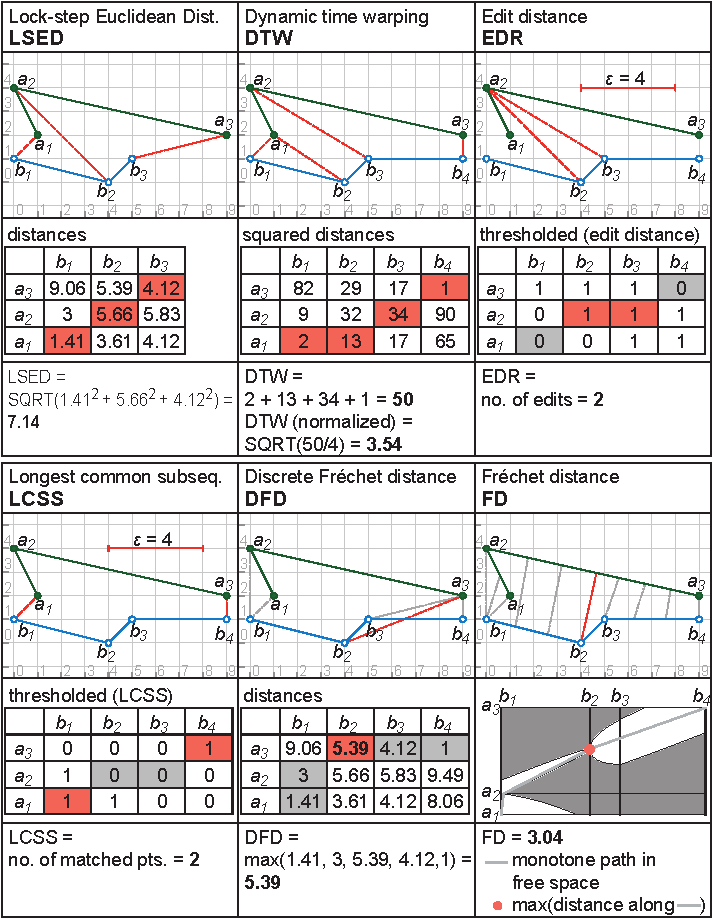
\includegraphics[width=100mm]{figures/Fig2}
\caption{Aligning two trajectories where $n$=3 and $m$=4 (except for LSED, where $n$=$m$=3) according to the various measures, along with a corresponding distance matrix or free-space diagram. The distances relevant for computing the respective similarity measures are added as dashed red lines in the figures and highlighted in red in the matrices, e.g distance $\dist(a_3,b_2)$ for DFD.}\label{fig:Traj_align}
\end{figure}

\subsection{Lock-step Euclidean distance (LSED)}

% Tests on Lock-step Euclidean distance will not be delivered here because of its .

%, with Lock-step Euclidean distance being the only measure mentioned that can reflect such similarity, for instance, by summing (in the discrete setting) or integrating (in the continuous setting) over time, or by taking the maximum distance over all times.

If  $n=m$ we can interpret the trajectories as points in the Euclidean space $\mathbb{R}^{2n}$ and take their Euclidean distance.

\begin{definition}
The lock-step Euclidean distance distance of $A$ and $B$ is defined as
\[
Eu(A,B) = \sqrt {\sum_{i=1}^n \dist_2^2(a_i,b_i)}\;.
\]
\end{definition}

A frequently used variant is the average distance between corresponding measurements:
\begin{equation}
Eu'(A,B) = \frac{1}{n}\sum_{i=1}^n \dist_2(a_i,b_i)\;.
\end{equation}
Alternatively, the maximum instead of the average distance can be used.

The definition above is most meaningful when there is a correspondence in time between the two trajectories.
That is, if $s_i = t_i$ for all $1 \leq i \leq n=m$, then LSED measures how far the trajectories are apart at corresponding times. In particular, $Eu'(A,B)$ is then the average distance at corresponding times.
If we assume uniform sampling in time, then the requirement $n=m$ corresponds to both trajectories having the same duration, i.e., $s_n - s_1 = t_n - t_1$. However, if both trajectories have the same duration but use different---possibly non-uniform--- sampling, then we can generalize these measures using interpolation:
\begin{equation}
Eu(A,B) = \frac{1}{n}\int_0^{s_n-s_1} \dist_2(A(s_1+t),B(t_1+t)) dt\;,
\end{equation}
where $A(t)$ and $B(t)$ are the locations of A and B, respectively, obtained by interpolation. Most commonly linear interpolation is used for this, i.e., for $s_i \leq t \leq s_{i+1}$ we have:

\begin{equation}
\label{eq:interpolated_traj}
 A(t) = a_{i} \frac{s_{i+1}-t}{s_{i+1}-s_i}  + a_{i+1} \frac{t -s_i}{s_{i+1}-s_i}\;.
\end{equation}

This interpolation assumes that the  object moves between two measurements with constant speed along a straight line; an alternative is to bound these distances only assuming an upper bound on the speed of movement~\citep{DBLP:conf/gis/BuchinP13}. All the distances above are easily computed in $O(n+m)$ time by scanning over the data once.

The Euclidean distance between two trajectories and its variants are widely used (cf.~\cite{VlachosGK02}). A key assumption underlying these measures is that the two trajectories are aligned in time. All of the following measures relax this condition: data points with different time stamps may be aligned as long as the alignment preserves the order of the points along the trajectories. For all of the measures the alignment is optimized according to certain criteria. The measures differ in the specific criteria.

\subsection{Dynamic time warping (DTW)}
Dynamic time warping is a classical dynamic-programming algorithm, originally used for speech recognition. DTW has been successfully applied to time series data since the work by \cite{BerndtC94}. Later, it became one of the most common methods for measuring similarity between trajectories. The following definition follows the one presented by \cite{ChenOO05}.

\begin{definition}
The dynamic time warping distance of A and B is is defined as
\[
\DTW(A,B) =
\left\{
	\begin{array}{ll}
		0  & \mbox{if A and B are empty} \\
		\infty  & \mbox{if A or B are empty (not both)} \\
		\dist_2^2(a_1,b_1) +
		\min( \\
	\DTW(A_{[2,n]},B_{[2,m]}), \\
			  \DTW(A,B_{[2,m]}),  \\
			\DTW(A_{[2,n]},B)) & \mbox{otherwise } \\
		\end{array}
\right.
\]
\end{definition}

\paragraph*{Matrix formulation}
For this algorithm and several of the following ones, it will be insightful to interpret the distance definitions in terms of paths in the distance matrix between the trajectory points, illustrated in Fig.~\ref{fig:Traj_align}, for two sample trajectories $A$ and $B$.
In the figure, the rows and columns of the matrix are laid out such that the squared distance between the first two points is at the lower left and the last two points at the upper right corner of the matrix.

%\begin{figure}[ht]
%\centering
%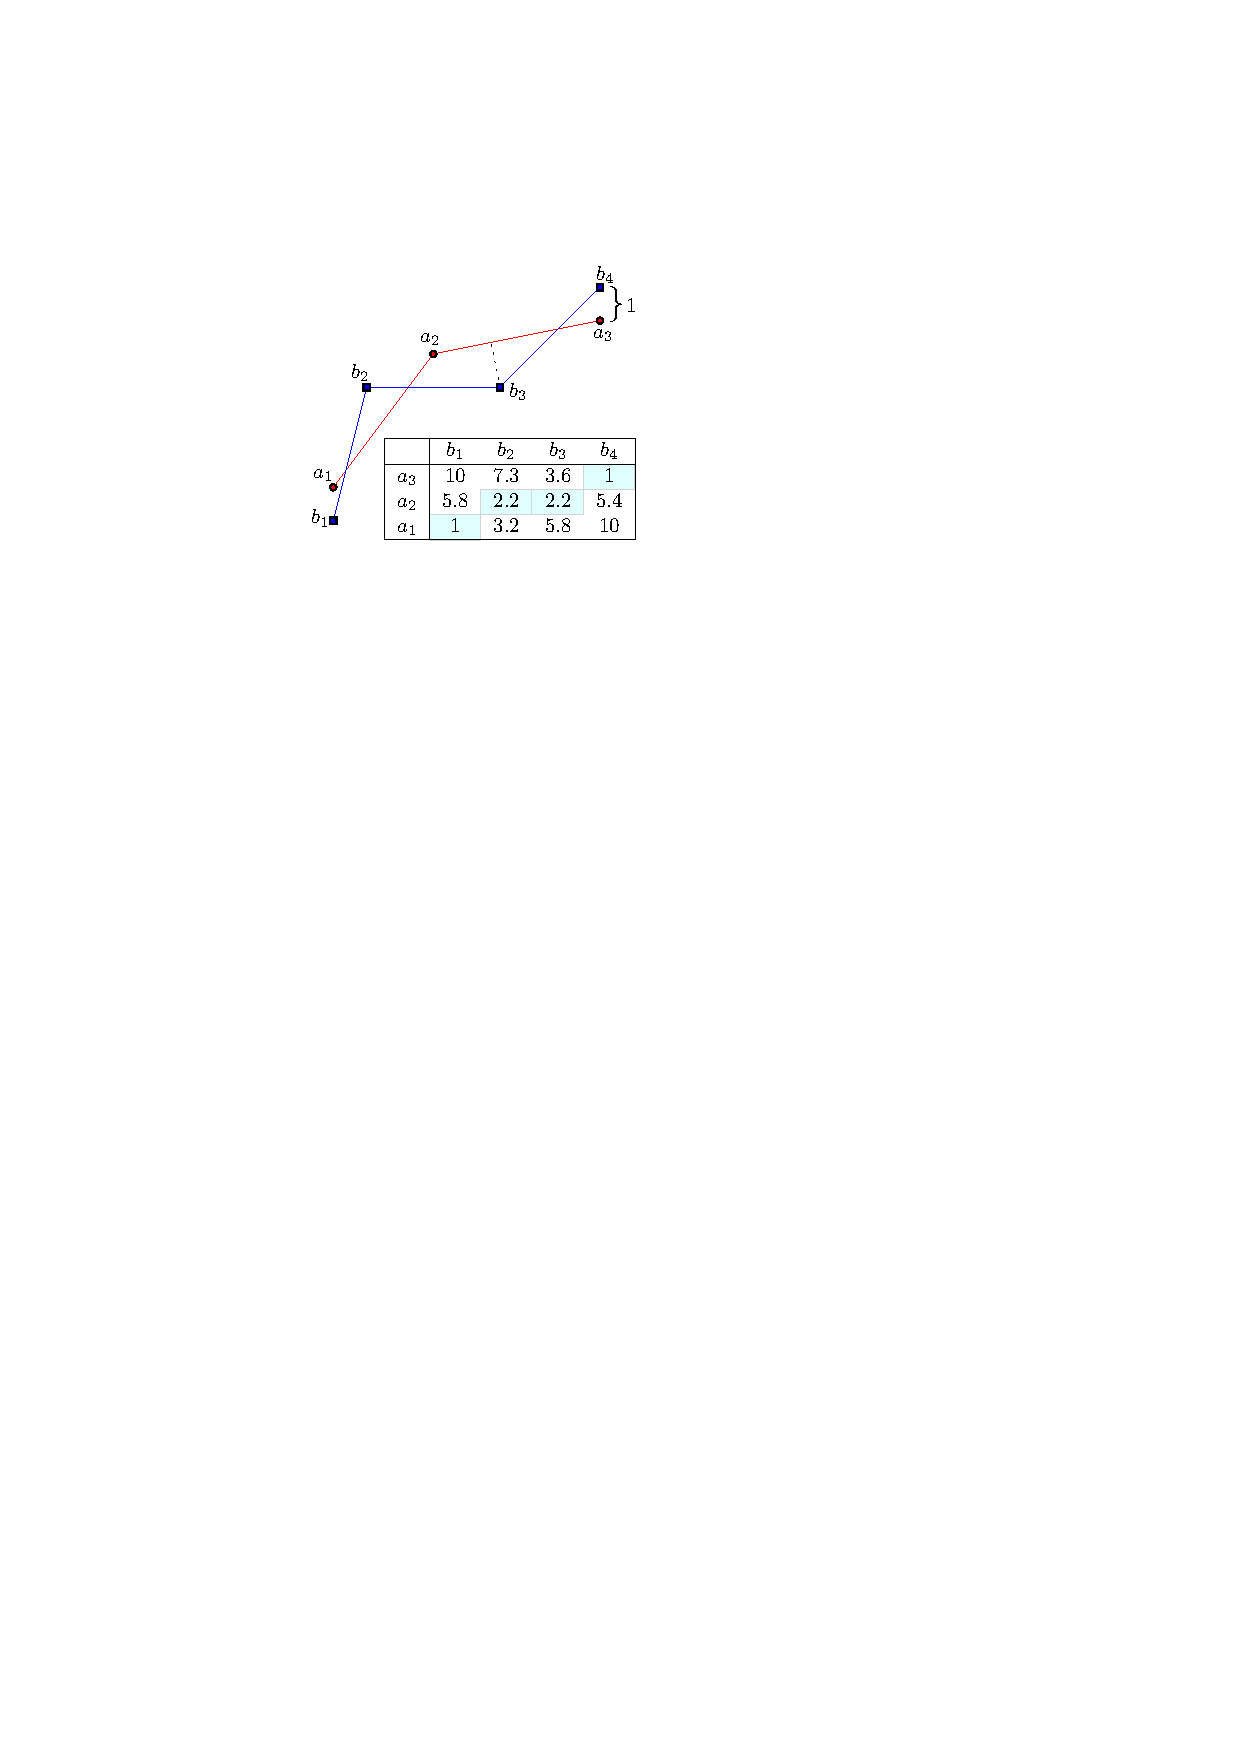
\includegraphics{figures/Fig1}
%\caption{Two trajectories and their distance matrix. In the distance matrix the optimal alignment according to DTW is highlighted.}\label{fig:DTW_eg} \end{figure}

Dynamic time warping can be seen as selecting a minimum cost path in the distance matrix.
More precisely, DTW selects a path from the lower left to the upper right corner of the distance matrix that minimizes the sum of squared distances. In the example, the resulting sum is $2 + 13 + 34 + 1
 = 50$. DTW is based on defining a cost for aligning two data points, namely the squared Euclidean distance between them.

From the point of view of walking along this path, from the lower left to the upper right corner, at each step DTW considers three possible moves: horizontal, vertical or diagonal.  More specifically, the options available are:
\begin{enumerate}
\item \textit{Match current pair of points, and move diagonally}: the cost of this move is equal to the squared distance between the pair of points.
\item \textit{Match current pair of points, and move up}: the cost is equal to the squared distance between the pair of points.
\item \textit{Match current pair of points, and move right}: the cost is equal to the squared distance between the pair of points.
\end{enumerate}

Another useful way to visualize the DTW approach is in terms of alignments. Each path in the distance matrix considered by DTW corresponds to an \emph{alignment} between the points of the two trajectories (red dashed lines, Fig.~\ref{fig:Traj_align}). 
Each cell in the path implicitly aligns one point of $A$ with one of $B$, that is, a path  through cell $(i,j)$, for $1 \leq i \leq n$ and $1 \leq j \leq m$, is implicitly aligning $a_i$ with $b_j$.

What characterizes a similarity measure like DTW is how the cost of a path is defined, since the cost of a path represents how well the two trajectories are aligned in that path. 
Following~\cite{ChenOO05}, in the definition above the cost of a path is the sum of the squared distances between all pairs of aligned points. 
However, DTW is also frequently used with other costs, e.g., turning angles, discussed in more detail at the end of this section.
It is also common to enforce additional constraints on the path, for instance enforcing similar time-stamps between aligned measurements (see, for example,~\citealp{keogh2005exact}).

\paragraph*{Normalization}
The DTW distance corresponds to a sum of squared distances between data points and depends on the number of data points used. This makes it difficult to compare DTW distances between different numbers of data points in each trajectory. In the experiments we therefore divide the DTW distance by $\max (m,n)$, which is (in the matrix formulation) the smallest number of cells that need to be visited. To obtain a more comprehensible 1D-distance measure, we additionally take the square root, that is, as normalized DTW distance we use $\sqrt{\DTW(A, B)/\max (m,n)}$, which produces $\sqrt{50/4}=3.54$ for the example in Fig.~\ref{fig:Traj_align}.

It might seem natural to normalize using the number of values in the sum (in terms of the matrix formulation: the number of cells visited) instead of $\max (m,n)$. This approach would however make the normalized distance dependent on the path in the matrix, assigning relatively smaller normalized distances to longer paths.

\paragraph*{Algorithm}
The dynamic time warping distance is computed using dynamic programming, meaning that in terms of the formulation above one can compute for every cell $(i,j)$ the cost of the best path to reach it. This computation requires constant time per cell, as a cell's cost can be computed based on the cost of the cell left, below, and diagonally (left-below), resulting in an overall quadratic, i.e., $O(nm)$, computation time.
In practice, this can often be reduced to linear time, by carefully avoiding the computation for cells that have no influence on the final result~\citep{keogh2005exact}.
To decrease the computation time further, deep neural network based models are developed to fit DTW measure, see for instance~\citep{zhang2019deep}.


\subsection{Edit distance (EDR)}
Originally proposed to measure how similar two strings of characters are, edit distances have been successfully used for trajectory similarity. Conceptually, edit distance makes the changes (``edits'') to a trajectory---for instance, deleting a data point---needed to morph it into another trajectory. Every edit comes at a cost. Here we present the variant proposed by \cite{ChenOO05}, known as \emph{edit distance on real sequence} (EDR). In this variant every edit has a unit cost, and the edit operations are either deleting a point, or aligning two dissimilar points.

\begin{definition}
The edit distance on real sequence (EDR) of $A$ and $B$ is defined as
\[
\EDR(A,B) =
\left\{
	\begin{array}{ll}
		n  & \mbox{if B is empty} \\
		m  & \mbox{if A is empty} \\
		\min( \\\EDR(A_{[2,n]},B_{[2,m]})+\mbox{penalty}(a_1,b_1), \\
			  \EDR(A,B_{[2,m]}) +1, \\
			\EDR(A_{[2,n]},B)+ 1) & \mbox{otherwise } \\
		\end{array}
\right.
\]

where $\mbox{penalty}(a_1,b_1)$ is 0 if $\dist_\infty(a_1,b_1) < \epsilon $, or 1 otherwise.
\end{definition}
The definition uses a parameter $\epsilon$ as a matching threshold distance (i.e., two points closer than $\epsilon$ are considered to match).
\paragraph*{Matrix formulation}
Similar to DTW, EDR searches for a minimum cost path in the distance matrix, although it uses a matrix where the cost is defined differently. 
The cost of the path is the number of horizontal, vertical, and diagonal steps, excluding diagonal steps for which the corresponding pair of points are considered to match (i.e., their distance is smaller than $\epsilon$). 
%As in DTW, there are three possible ways to move in the path towards the upper right corner:

%\begin{enumerate}
%\item \textit{Match current pair of points, and move diagonally}: The cost of this move depends on whether the current pair of points are considered to match (i.e., their distance is smaller than $\epsilon$).
%In the former case there is no cost, in the latter the cost is one unit.
%\item  \textit{Move right}: This costs one unit.
%\item  \textit{Move up}: The cost is one unit.
%\end{enumerate}

It is important to note that in EDR costs are thresholded to 0 if the current pair of points match, whereas in all other situations the cost is 1, irrespective of the distance between the current pair of points. This results in the \emph{distance threshold matrix}, a Boolean matrix as shown in Fig.~\ref{fig:Traj_align}.
However, non-thresholded versions also exist.
For instance, EDR itself is an adaptation of a measure proposed by \cite{NgC04} called \emph{edit distance with real penalty} (ERP). Instead of penalizing by 1 every time two elements do not match, ERP penalizes with the squared distance between the non-matching elements.

%[\texttt{Caption of Fig. 3}: boolean matrix for thresholded distances for trajectories from Fig.~1.]
%\begin{figure}[ht]
%\centering
%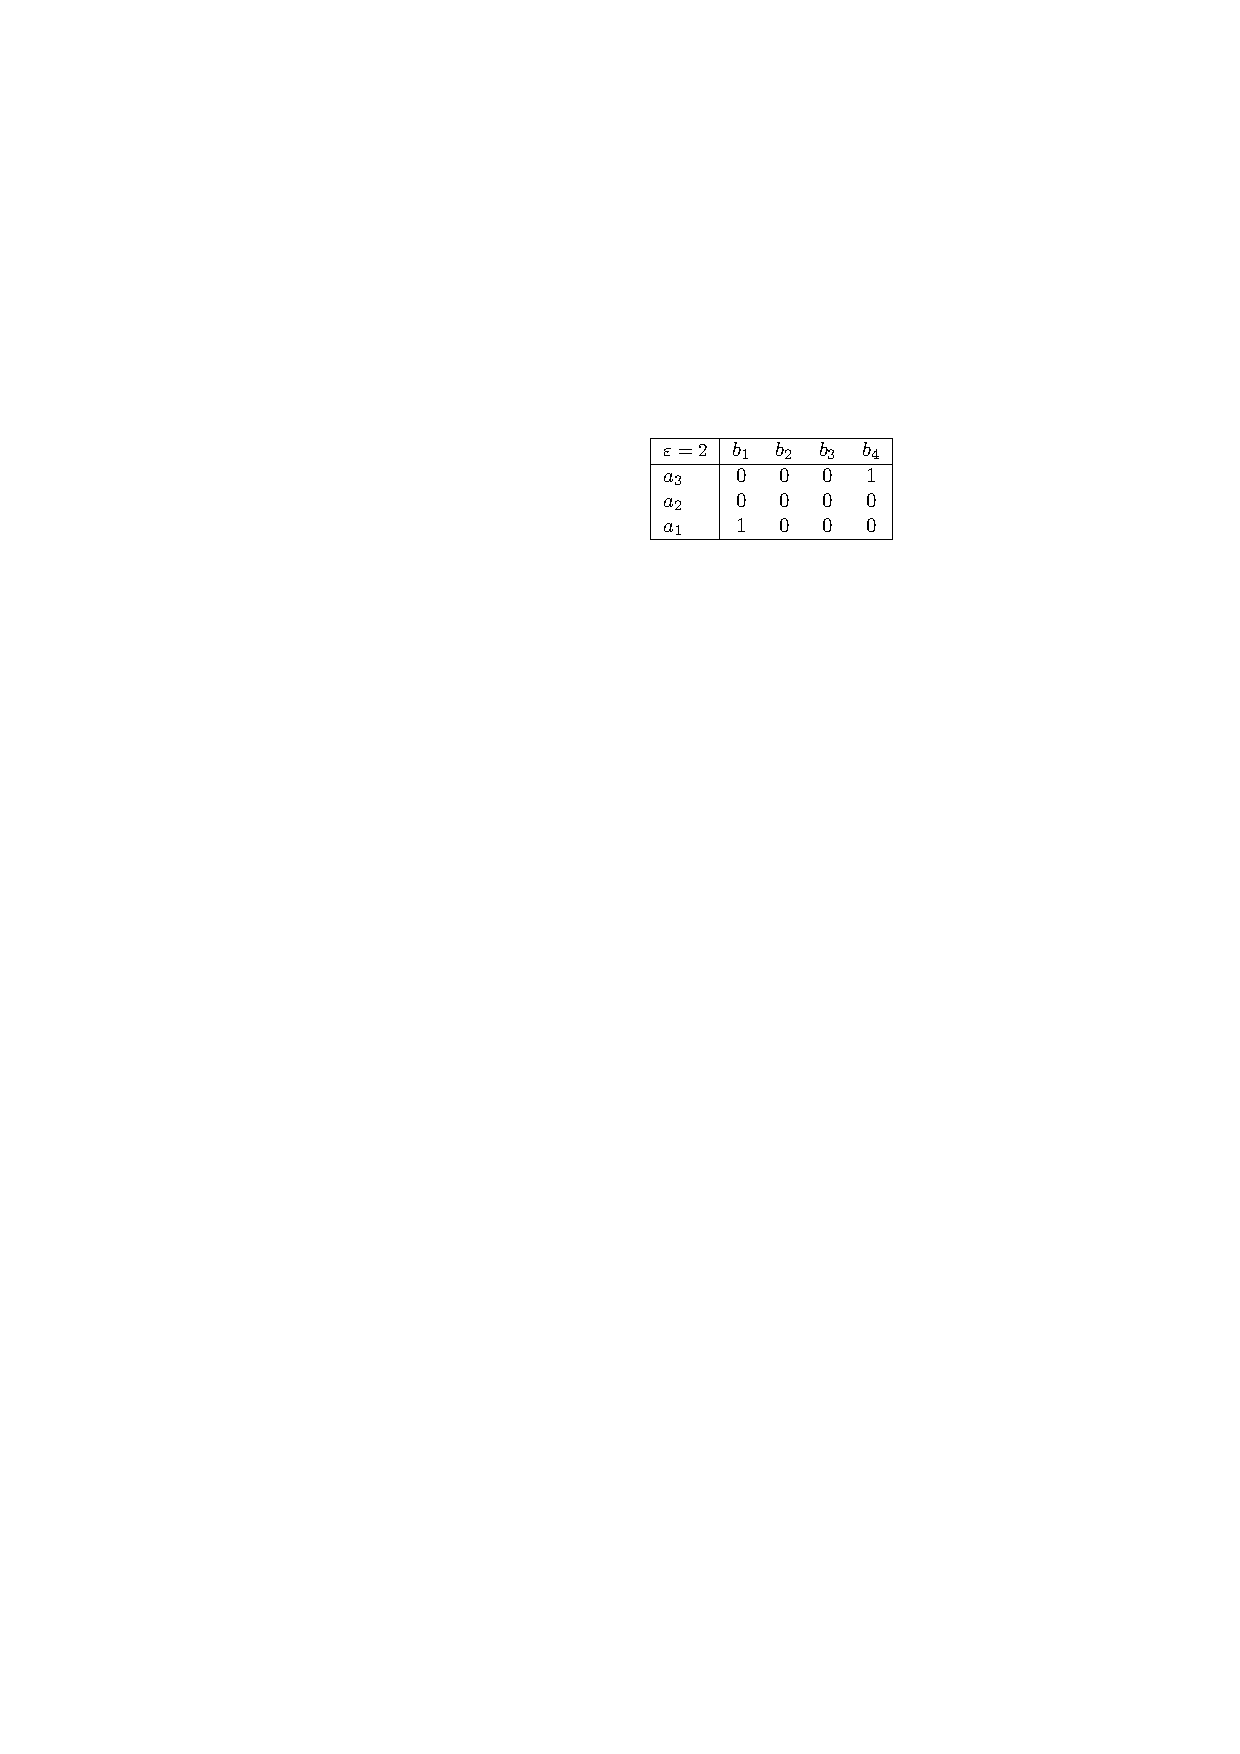
\includegraphics{figures/Fig3}
%\caption{Boolean matrix for thresholded distances for trajectories from Fig.~1.}\label{fig:Bool_matrix}
%\end{figure}

In terms of alignments, EDR defines the cost of a path as the number of aligned points that are not considered a match.

\paragraph*{Algorithm}
Computing edit distances can be implemented in the same way as DTW and therefore take quadratic time, $O(nm)$, in the worst case.


\subsection{Longest common subsequence (LCSS)}
Longest common subsequence measures try to capture how well two trajectories match by measuring the length of the longest point sequence that they have in common. LCSS measures are closely related to edit distances, defined as follows after \cite{VlachosGK02}.

\begin{definition}
The length of the longest common subsequence between $A$ and $B$ is defined as
\[
\LCSS(A,B) =
\left\{
	\begin{array}{ll}
		0  & \mbox{if A or B is empty} \\
		1+\LCSS(A_{[1,n-1]},B_{[1,m-1]}) & \mbox{if } \dist_\infty(a_n,b_m) < \epsilon  \mbox{ and } \\ &|n-m| \leq \delta \\
		\max( \LCSS(A_{[1,n-1]},B), \\ \LCSS(A,B_{[1,m-1]})) & \mbox{otherwise } \\
		\end{array}
\right.
\]
\end{definition}

The definition uses two parameters, $\delta$ and $\epsilon$.
As in EDR, $\epsilon$ is a matching threshold distance (i.e., two points closer than $\epsilon$ are considered to match).
Additionally, $\delta$ controls how far in time (specifically, in timesteps) two matching points can be, in order to align the trajectories in time.
However, it should be noted that $\delta$ is not specific to LCSS, and could be added to any of the other measures.

\paragraph*{Matrix formulation}
%\rodrigo{Mention that we keep this redundant formulation  on purpose  for this and the following methods because it is interesting}
LCSS also looks for a path in its distance matrix (Fig.~\ref{fig:Traj_align}), although with a few differences with respect to the previous measures.
First, the path is searched in the opposite direction: from the upper right to the lower left corner. This is an arbitrary decision: it is easy to modify the formula to go in the same direction as DTW and EDR. But we preferred here to follow the original formulation from~\cite{VlachosGK02}.
The salient difference in LCSS is that the goal is to find a path of \emph{maximum} score, with the objective to maximize the number of matched points. The score of a path is the number of diagonal steps, where diagonal steps are only allowed if points are similar. 

%As before, there are three possible ways to advance:
%\begin{enumerate}
%\item \textit{Match current pair of points, and move diagonally}: To be considered a match, the pair of points cannot be further than $\delta$ timesteps away. This movement gains (costs) one unit
%\item \textit{Move left}: This movement results in no gain (cost).
%\item \textit{Move down}: This movement results in no gain (cost).
%\end{enumerate}

In common with to EDR, LCSS is thresholded, meaning whether the point pairs match or not matters, but not the magnitude of difference. In terms of alignments, LCSS defines the value of a path as the number of alignments considered a match, making LCSS a measure that is somewhat complementary to EDR. Indeed, ignoring that one measure minimizes a cost and the other maximizes a score, the difference between LCSS and EDR is subtle: EDR allows diagonal steps for dissimilar points (at a cost), while LCSS does not. 

\paragraph*{Algorithm}
As before, LCSS can be implemented using dynamic programming, and therefore takes quadratic time, $O(nm)$, in the worst case.

% Commenting out part about how to make it a distance
\iffalse
Now we can define a similarity function based on LCSS.

\begin{definition}
LCSS-based similarity measure and distance definitions for two trajectories $A$ and $B$.
\[
S(A,B)=\frac{LCSS(A,B)}{\min(n,m)}
\]
\[
D(A,B)=1-S(A,B)
\]
\end{definition}

\cite{VlachosGK02} also give a second similarity measure that is invariant to translations, but here we only present the simplest version.
\fi


\subsection{Discrete Fréchet distance (DFD)}
Proposed by \cite{Wien94computingdiscrete}, DFD can be seen as a version of DTW that takes the \emph{maximum} distance between aligned points along the path. This is in contrast to DTW, which considers the \emph{sum} of all squared distances.

\begin{definition}
The discrete Fr\'echet distance of $A$ and $B$ is defined as
\[
\DFD(A,B) =
\left\{
	\begin{array}{ll}
		0  & \mbox{if A and B are empty} \\
		\infty  & \mbox{if A or B are empty (not both)} \\
		\max( \dist_2(a_1,b_1),
		\min( \\
	\DFD(A_{[2,n]},B_{[2,m]}), \\
			  \DFD(A,B_{[2,m]}),  \\
			\DFD(A_{[2,n]},B)) & \mbox{otherwise } \\
		\end{array}
\right.
\]
\end{definition}

\paragraph*{Matrix formulation}
Similar to DTW and EDR, DFD searches for a minimum cost path in the distance matrix, from the lower left to the upper right corner (Fig.~\ref{fig:Traj_align}). As in DTW, the cost of a pair is measured by taking the Euclidean distance.

%, and there are three possible ways to advance:
%
%\begin{enumerate}
%\item \textit{Match current pair of points, and move diagonally}: The cost is equal to the distance between the pair of points, only if it is greater than or equal to the cost of the rest of the path.
%\item \textit{Match current pair of points, and move up}: The cost is equal to the distance between the pair of points, only if it is greater than or equal to the cost of the rest of the path.
%\item \textit{Match current pair of points, and move right}: The cost is equal to the distance between the pair of points, only if it is greater than or equal to the cost of the rest of the path.
%\end{enumerate}

%\kevin{Check whether we consistently use alignment.}
In terms of alignments, DFD defines the cost of a path as the maximum over the distances between all pairs of aligned points. Note that taking the squared distance instead of the distance would result in the same optimal paths. Essentially, DFD's difference to DTW is that it takes the maximum instead of the sum of the distances between all pairs of aligned points.

\paragraph*{Algorithm} As before, DFD can be implemented using dynamic programming, resulting in an $O(nm)$-time algorithm.


\subsection{Fr\'echet distance (FD)}
All the distance measures above are discrete, in the sense that they only align the measured locations $a_i$, $b_i$. This can potentially lead to problems for non-uniform sampling. In this  section we present the Fr\'echet distance~\citep{ag-cfd-95}, which is also based on the maximum distance between the alignments, as DFD. However, in FD the alignments considered are \emph{continuous}, meaning that they are taken between all points in both trajectories, by using the interpolated trajectories $A(s), B(t)$ (defined as in Formula~\ref{eq:interpolated_traj}).

\begin{definition}
The Fr\'echet distance between $A$ and $B$ is defined as
\[
F(A,B) = \inf_{\sigma} \max_{t \in [s_1,s_n]} \dist_2(A(t),B(\sigma (t))),
\]

where the infimum is taken over all continuous, strictly monotone-increasing functions $\sigma \colon [s_1,s_n] \rightarrow [t_1, t_m]$ (i.e., all continuous alignments).
\end{definition}

%This can be interpreted as the continuous version of the discrete Fr\'echet distance. Indeed, continuous versions of the other measures discussed above have also been proposed.

\paragraph*{Algorithm} Algorithms to compute the Fr\'echet distance usually solve as a subroutine the decision problem: to decide whether the Fr\'echet distance is smaller than a given $\epsilon > 0$. Given an algorithm for the decision problem, the Fr\'echet distance can be approximated by using a binary search over $\epsilon$. A more complex search procedure, such as parametric search, can be used to compute the Fr\'echet distance exactly~\citep{ag-cfd-95}.

The Fr\'echet decision problem can be solved by a dynamic programming algorithm. Consider the so-called \emph{free-space diagram} in Fig.~\ref{fig:Traj_align} (bottom right). The free-space diagram is the continuous analog to the distance threshold matrix used for the edit distance and LCSS. In the free-space diagram the vertical axis corresponds to the parameter space of $A$ and the horizontal axis to the parameter space of $B$. Thus, the point $(s,t)$ in the diagram corresponds to the pair of points $(A(s), B(t))$. The free space for a given $\epsilon > 0$ is the set of points $(s,t)$ with the property that the distance between $A(s)$ and $B(t)$ is at most $\epsilon$.

In Fig.~\ref{fig:Traj_align}, the free-space diagram for $\epsilon \approx 3.04$ is the white-colored region. The Fr\'echet distance is at most $\epsilon$ if and only if there is a path from the lower-left corner to the upper-right corner that goes through the free-space and is monotonically increasing in both coordinates (shown in light grey). To compute whether such a path exists we can incrementally compute the part of the free-space diagram that is reachable by such a path. This results in an $O(mn)$-time algorithm for the decision problem. Computing the exact Fr\'echet distance then requires an additional $O(\log (mn))$ factor for the parametric search~\citep{ag-cfd-95}. In the example of Fig.~\ref{fig:Traj_align} the exact Fr\'echet distance is approximately 3.04 as the white region would disconnect when $\epsilon$ is decreased any further. The corresponding alignment is shown as a dashed red line.

\section{Discussion of conceptual and theoretical analysis}
Following our pen-and-paper conceptual and theoretical analysis, and before moving on the the experimental exploration, this section summarizes the key differences between the similarity measures.

% Metric: Yes to: LSED, DFD, FD, perhaps ED (\emph{edit distance with real penalty}~\cite{NgC04}), but not EDR; No to DTW, LCSS, EDR
% Continuous: Yes to FD; maybe LCSS (partial Fr\'echet distance~\cite{bbw-09}); maybe summed or average Fr\'echet distance~\cite{b-cfdts-07} and ~\cite{efrat2007curve}, continuous version of DTW; no LSED, DFD, ED.
% Absolute time: LSED; all others relative time.
% Absolute space: No for all with transformations; A no for all except LSED and FD using transformation invariant properties
% Computational differences
% This is done by first making an analysis of the ways in which the measures differ before discussing the decision process involved in selecting one particular measure over the others.

% Recall that most of the measures discussed align two trajectories and in this way take time into account qualitatively.


\subsection{Metric versus non-metric}

LSED, DFD, and FD are metrics.  DTW, LCSS, and EDR are not metics because:
\begin{itemize}
\item DTW does not obey the triangle inequality;
\item LCSS does not measure difference (instead measuring, to some extent, similarity), although variants that satisfy some weaker conditions can be defined~\citep{VlachosGK02}; and
\item EDR does not fulfill two of the conditions of a metric, namely the identity of indiscernibles ($D(A, B) = 0$  if and only if   $A = B$)  and the triangle inequality ($D(A, B) + D(B, C) \geq D(A, C)$).
\end{itemize}
However, in general edit distance may be a metric, including some variants of edit distance used for time-series analysis, such as \emph{edit distance with real penalty}~\citep{NgC04}.

\subsection{Discrete versus continuous}

Fr\'echet distance (FD) is the only one of the similarity measures considered here that is continuous. FD works by finding a continuous alignment: one between the complete path of both trajectories, not just between trajectory fixes. Continuous measures are more natural when the interpolated values between trajectory points are relevant. Moreover, continuous measures are better suited to handling trajectories with differing sampling rates and gaps.

To illustrate, consider how the discrete versus continuous measures change in the presence of a data gap, leading to one long trajectory segment. Discrete measures will only consider the endpoints of that segment, producing an increase in the similarity measure. In the case of measures based on the sum of distances (e.g., LSED, DTW, EDR, LCSS), this increase may average out. However, measures that are based on the maximum distance (e.g., DFD) will drastically increase. In contrast, a continuous measure is likely to show the smallest effect in the presence of gaps or different sampling rates, as long as the points on the interior of long segments can be aligned to nearby points on the other trajectory.

Implementing a continuous measure does present additional computational challenges, as opposed to the relative simplicity of a discrete measure. However, the worst-case running time of the FD is only slightly worse than that of the other measures. Indeed, just as FD was described as a continuous version of the DFD, continuous versions of some other measures have also been defined. The so-called \emph{partial Fr\'echet distance}~\citep{bbw-09} is the continuous analogue of LCSS. For a given $\epsilon >0$, the partial Fr\'echet distance aligns two trajectories to maximize the parts that have distance at most $\epsilon$, measuring the overall length of these parts. The summed or average Fr\'echet distance is a continuous version of dynamic time warping, and aligns the trajectories as to minimize the average distance between matched points~\citep{b-cfdts-07}. Continuous versions of dynamic time warping using other measures for the pairwise distance between matched points have also been considered~\citep{efrat2007curve}.


\subsection{Relative versus absolute time}
LSED is the only similarity measure considered that compares measurements at corresponding times (possibly after an absolute time shift). Common to all of the other similarity measures discussed, DTW, ED, LCSS, DFD, and FD, is the principle of temporally aligning the two trajectories by aggregating the local costs (i.e., the cost of the temporal alignment between each pair of points). The key differences between measures often lie in the details of how this is done. For instance, DTW and DFD fundamentally differ only on whether to take the sum (DTW) or the maximum (DFD) of the local costs. This difference has knock-on impacts on how local time differences influence the measure. For instance, since DTW adds up the distance values of the cells visited (in the matrix formulation), it is of advantage to visit fewer cells, and therefore to take diagonal steps unless there is a bigger gain in terms of the local cost by taking horizontal/vertical steps. For all the measures, how much local variation in time is allowed can be restricted by restricting the path in the distance matrix to cells close to the diagonal (or more generally, close to the path that corresponds to a perfect alignment in time). The extreme case where the path is completely restricted  corresponds to LSED (or a variant thereof).


\subsection{Relative versus absolute space}

The distance measures considered above align trajectories in time to minimize absolute Euclidean distances. However, depending on the application, relative distance may be more important. This is addressed in two different ways. The first approach is to take one of the measures above and optimize it under a suitable set of transformations, e.g., translations. That is, if $D(A,B)$ is a distance measure between trajectories $A$ and $B$, one would consider $\min \{d(A,B + \tau)\;|\; \tau \in T \}$, where $T$ is the set of two-dimensional translations. This minimization problem is typically computationally expensive (see for example~\citealp{VlachosGK02}), and often solved by sampling the space of transformations~\citep{as-sm-12}. The second approach is much simpler. Instead of using Euclidean distances, an alternative measure that is invariant under a suitable set of transformations is used. Common choices for this alternative include heading (translation-invariant) and turning angle (translation- and rotation-invariant). For instance, one can use DTW with turning angles instead of squared Euclidean distances. 
%To that end, the turning angle must be defined for each point $a_i$. This is usually done by considering points $a_{i-1}$ and $a_{i+1}$, and computing the angle between vectors $\overrightarrow{a_{i-1} a_{i}}$ and $\overrightarrow{a_{i}a_{i+1}}$. 
Note that the use of measures such as heading or turning angle complicates the application of continuous similarity measures such as FD, since it would require to interpolate heading or turning angle between trajectory points. 
%This is, in general, hard to do in a meaningful way; for instance, turning angle is always zero between points if linear interpolation is used.

\subsection{Computational efficiency}

Regarding efficiency, the simplest and fastest measure discussed is LSED, as it only requires processing the input trajectories once, which takes $O(n+m)$ time. Fr\'echet distance is least efficient, but also the subject of considerable recent efforts to improve efficiency~\citep{bringmann2019walking}.
The dynamic programming-based measures (DTW, EDR, LCSS and DFD) require $O(nm)$ time in their standard formulations.
The dynamic programming approach is also easy to implement, and is almost identical for all four measures.
Theoretical improvements for some of these measures are possible \citep{DBLP:conf/icde/2002,bbmm-fswd-14,Masek198018}.
However, these are marginal improvements in practice and come at the cost of increased complexity of implementation.
Approximating a similarity measure can also yield faster computation. For instance, limiting how much local time-shifting is allowed restricts the search to a smaller portion of the distance matrix (or free space diagram for the Fr\'echet distance) close to the diagonal. 

\subsection{Outliers}

One final important difference between the various measures is worth highlighting: tolerance to outliers. Generally, measures that use the maximum distance between matched points (such as FD and DFD) emphasize large distances and are therefore more sensitive to outliers than measures that use the sum of distances (or the sum of squared distances). Thresholds (as used in the EDR and LCSS) can be useful for dealing with outliers as they allow for the assignment of a uniform cost to pairs that are matched but have a distance larger than the threshold. In this sense, LCSS can be interpreted as the measure that minimizes the number of points that need to be classified as outliers to perfectly align the remaining trajectories. This, however, comes at the cost of introducing the threshold as an additional parameter.

	
\section{Experiments}

Complementing the conceptual and theoretical analysis above, this section explores trajectory similarity through experiments with real data, to aid distinguishing between differences which may be theoretically important, but practically less relevant. To throw light on the widest range of practical scenarios, we selected two benchmark trajectory data sets with sharply contrasting properties: vehicle movements through a transportation network, and trajectories capturing the behavior of coastal wading birds.


\subsection{Data sets}
\label{sub:data sets}

The Dublin bus GPS sample data~\citep{DublinBus} was selected as our first data set.  This data set is especially suitable for separating spatial and temporal impacts, because the trajectories can be fixed in one dimension and varied in the other. For example, a group of bus trajectories from the same bus route taken at different periods of a day can be identical in their spatial path, but have quite different temporal features. 

A representative subsample of bus trajectories were extracted from four weekdays (2nd, 3rd, 4th, and 7th of January 2013) and 8--9am, 1--2pm, and 8--9pm time blocks. This selection mechanism allows trajectories to be grouped based on temporal similarity as well as spatial similarity. Trajectory segments at the start or the end of a trajectory, where the bus was considered to be stationary, were removed as such a high level of similarity would likely dominate any similarity measures used. Two example pairs of trajectories are shown in Fig~\ref{fig:eg_bus}.

\begin{figure}[ht]
	 \centering
	 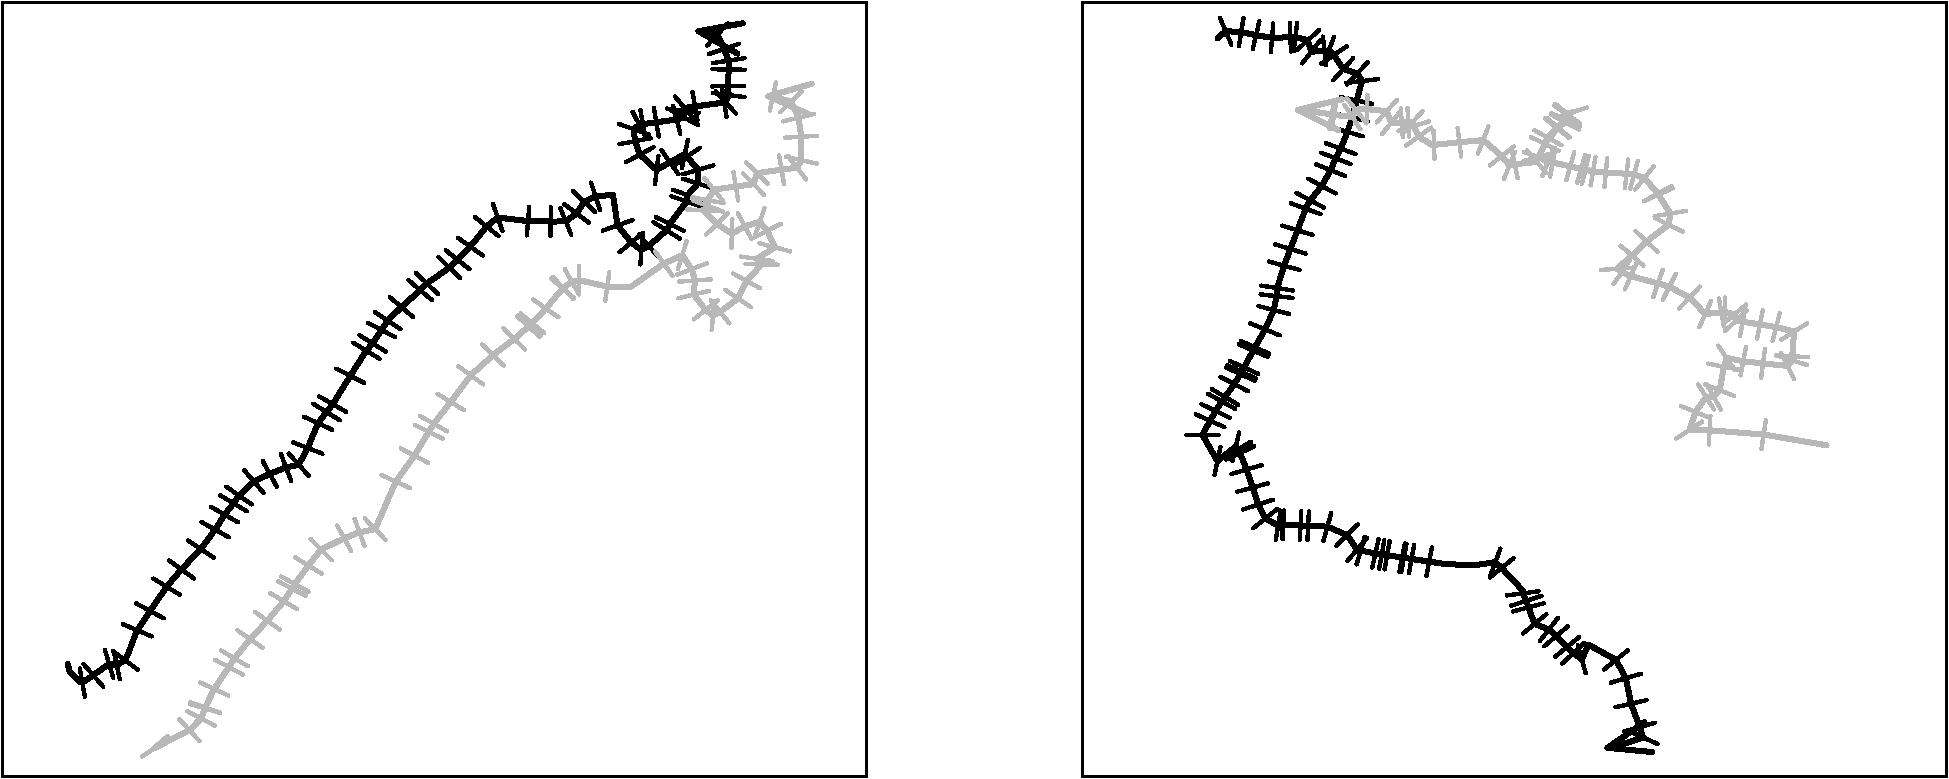
\includegraphics[width=120mm]{figures/busRoutesComparison}
	 \caption{Example bus trajectories. The left pair shows trajectories of the same bus route collected at the same time but on different days; the right pair shows trajectories with different routes and different times. Grey trajectories have been displaced for clarity.}
	 \label{fig:eg_bus}
\end{figure}

The second data set concerned GPS trajectories of oystercatchers, annotated with bird activities~\citep{shamoun2012sensor}. This data set was chosen to support comparisons between trajectories arising from different behaviors or activities. Specifically, trajectories annotated as \textit{flight} and \textit{foraging} were extracted for our analysis. A minimum trajectory length of three fixes was set to exclude trajectories that are too short to clearly indicate any embedded activity.

This data set is especially suitable for exploring similarity of trajectories transformed in time and space, as trajectories reflecting the same activity may occur in different locations, direction, and speeds. Distinctive features of trajectories make the different behaviors distinguishable. For example, oystercatchers are more likely to make sudden turns when they are foraging compared to cases when they are simply flying (Fig.~\ref{fig:illu_flight_forage}). An underlying assumption of some of our experiments is that the spatiotemporal characteristics of the behaviours are invariant under certain spatial or temporal transformations. 

\begin{figure}[ht]
	\centering
	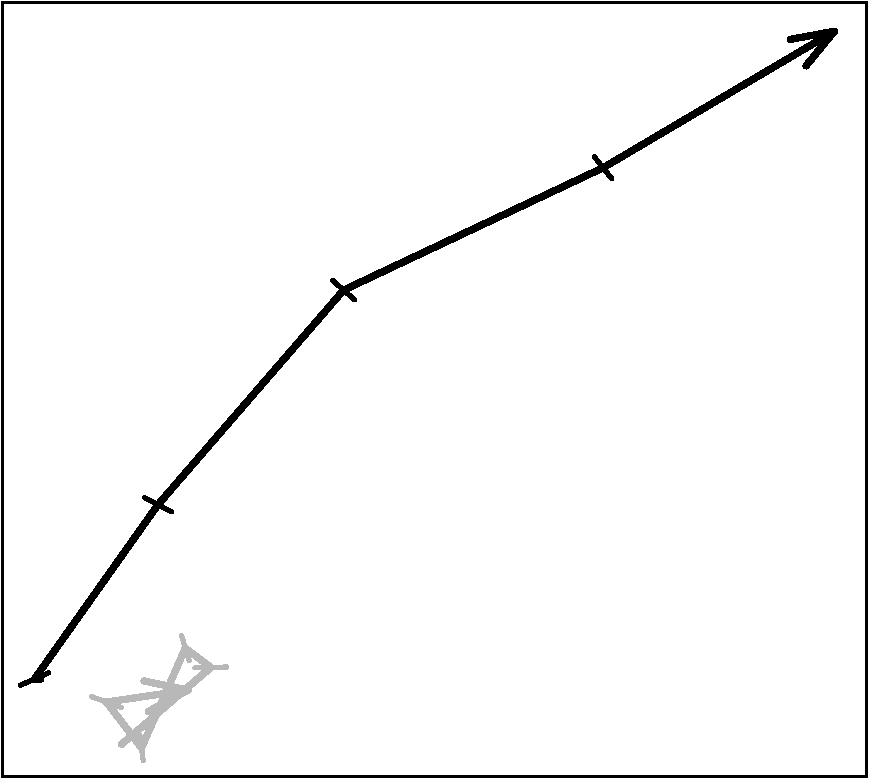
\includegraphics[width=60mm]{figures/birdComparison}
	\caption{One trajectory of flight (black) and one trajectory of foraging (gray)}
	\label{fig:illu_flight_forage}
\end{figure}


\subsection{Experiment 1: Verification and baseline}
\label{par:experiment_1}
Our first experiment examined the similarity measures when applied to a single high resolution trajectory under different transformations (Fig.~\ref{fig:sample bus}). A base trajectory was created by regular sub-sampling from the raw data (Fig.~\ref{fig:sample bus}a). Obviously, we expect all trajectory measures to find maximum similarity when trajectories are identical, and such a comparison can be seen as a trivial verification of the implementation of our code.  We then calculated similarity under the following conditions:

\begin{enumerate}
\item A temporal transformation, where points were sub-sampled from the original trajectory with an increasing temporal interval, clustering points towards the (temporal) beginning of the trajectory (Fig.~\ref{fig:sample bus}b);
\item A spatial transformation where the base trajectory was rotated slightly about its origin (Fig.~\ref{fig:sample bus}c); and
\item A spatiotemporal transformation where both temporal and spatial transformations  above were applied (Fig.~\ref{fig:sample bus}d).
\end{enumerate}

\begin{figure}[ht]
	 \centering
	 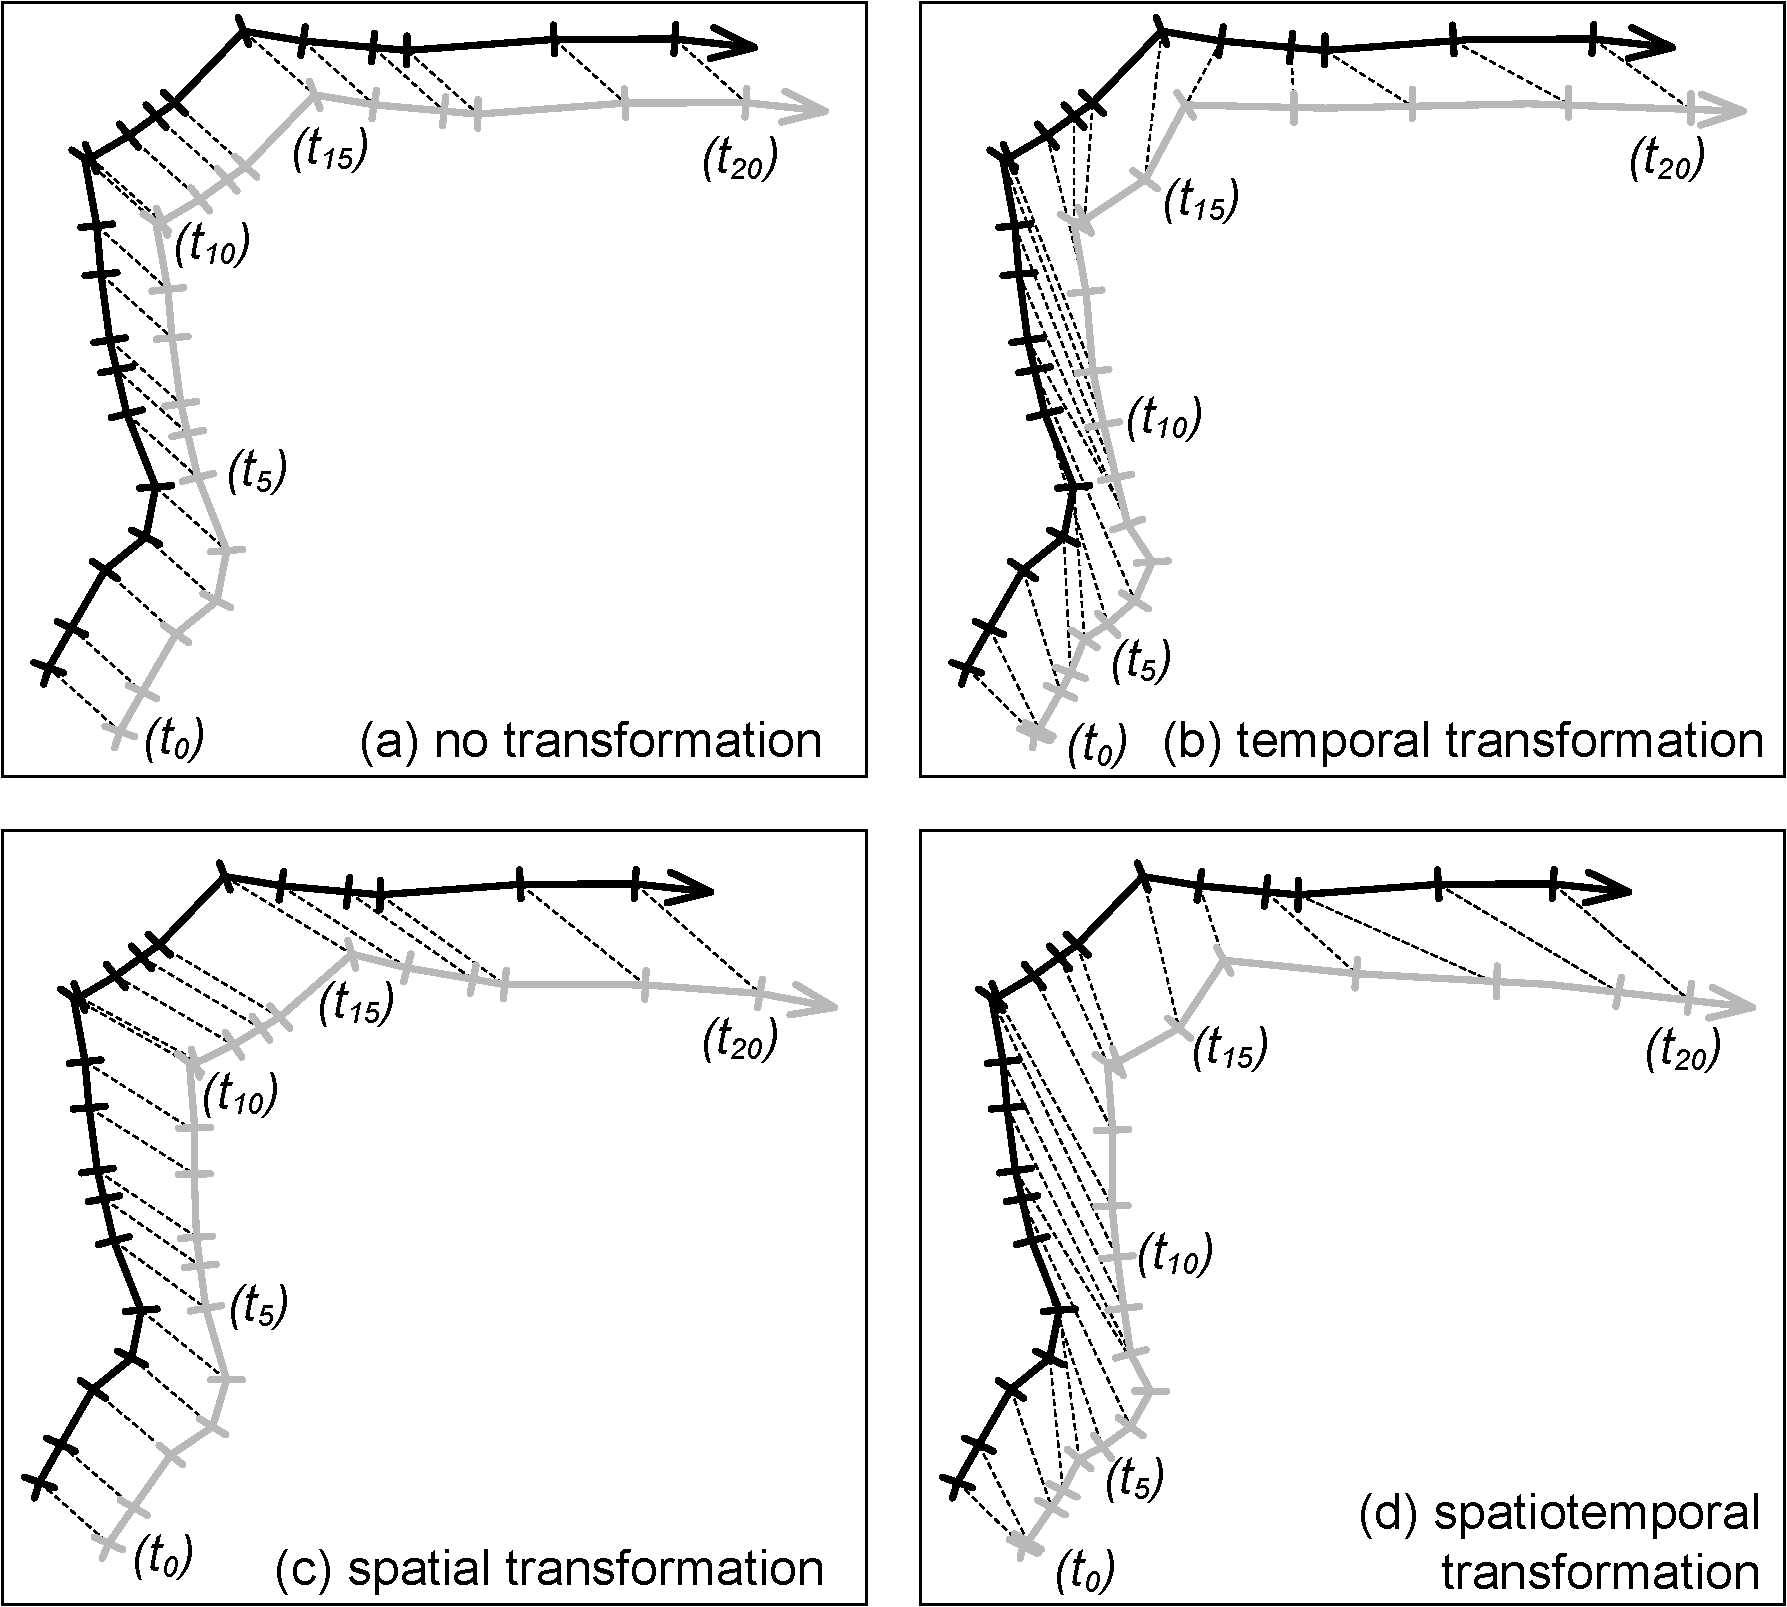
\includegraphics[width=110mm]{figures/trajectoryComparisons_V3}
\caption{Trajectory comparisons between one bus trajectory and its variations}
%(a) no transformation, (b) temporal transformation, i.e., measurements are temporally shifted towards one the begin of the trajectory, (c) spatial transformation, i.e., the gray trajectory has been rotated, and (d) spatiotemporal transformation, i.e., the combination of both the spatial and the temporal transformation.}	
\label{fig:sample bus}	
\end{figure}

In this experiment we are interested in the ordering of results within and between similarity measures. In other words, are the same trajectory pairs always more similar, irrespective of the similarity measure used? Or, as we expect from our theoretical analysis, are some measures more sensitive to spatial or temporal transformations than others?

\subsection{Experiment 2: Bus routes}
\label{par:experiment_2}
Our second experiment aimed to explore the behavior of different similarity measures on real trajectories constrained in a network space. Here, we assumed that spatial behavior, while not identical, is very similar for repeated instances of the same route. Temporal behavior, however, may vary greatly (i.e., from variations in traffic flow) based on the time of day. A key question then is: which similarity measures are better suited to discriminating between trajectories paired from different categories? We chose two dimensions along which to characterize trajectories: spatial similarity, where we select trajectories according to individual bus routes; and temporal similarity, where we select trajectories from the three sampled time periods (8--9am, 1--2pm, and 8--9pm, all on weekdays). These criteria were then used to randomly select 36 pairs of trajectories to test four scenarios:
\begin{itemize}
\item \emph{SameSame}: Pairs of trajectories along the same route in the same temporal window.
\item \emph{SameRoute}: Pairs of trajectories along the same route in different temporal windows.
\item \emph{SameTime}: Pairs of trajectories along different routes in the same temporal window.
\item \emph{DiffDiff}: Pairs of trajectories along different routes in different temporal windows.
\end{itemize}

These four scenarios capture the essential spatial and temporal dimensions of trajectory similarity of tracking data in network space. We hypothesize that similarity measures will be able to discriminate between trajectories along these dimensions.

\subsection{Experiment 3: Bird behaviours} % (fold)
\label{par:experiment_3}
In Experiment 3 our aim was to assess trajectory similarity with respect to existing behavioral labels (flight and foraging). We hypothesized that similarity measures should be able to discriminate between such behaviors. In this experiment, pairs of trajectories were selected randomly from labeled foraging behavior and from all of the small number of available flight trajectories to build the following comparison sets:

\begin{itemize}
\item \emph{FlyFly}: Pairs of trajectories labeled as flight.
\item \emph{FlyForage}: Pairs of trajectories labeled as flight and foraging.
\item \emph{ForageForage}: Pairs of trajectories labeled as foraging.
\end{itemize}

These comparisons are a typical example of trajectory similarity comparisons in a between-subjects experiment in ecology, where the aim is to describe animal behaviors using GPS tracks. Since such behavioral patterns need not take place within the same space, and we are interested in the general properties of the trajectories, a necessary first step is a spatial transformation (translation and rotation) to align trajectories. All trajectories were translated such that their origins were identical, and rotated so that the angle formed between the first and last point in every trajectory was 45 degrees. We hypothesized that similarity measures would capture differences between behavioral patterns through spatial behavior.


\subsection{Experiment 4: Buses vs Birds}
\label{par:experiment_4}
In any experiments comparing methods, it is important to consider straightforward baselines that are easy to interpret. Since the two data sets used exhibit very different properties, another experiment with transformation in space allowed was designed to compare two more general activities---bird activity and bus activity.
As the bird and bus trajectories lie far away from each other, transformation in space and time was utilized to enable comparison.
The similarity measures were then performed on three types of trajectory pairs:

\begin{itemize}
\item \emph{BirdBird}: Pairs of bird trajectories.
\item \emph{BusBird}: Pairs of bird and bus trajectories.
\item \emph{BusBus}: Pairs of bus trajectories.
\end{itemize}

Based on this pairing schema, a random set of both bird and bus trajectories were used to examine whether bus and bird are distinguishable based solely on their movement patterns.


\subsection{Measure normalization}\label{sec:measurenormalization}
As the trajectories used in the experiments can vary dramatically in length, a direct comparison of similarity measures is not possible. In order for all similarity measures to be compared within the same categories, and between inter-category groups, LCSS, DTW, and EDR similarity values needed to first be normalized. LCSS was normalized by the shortest trajectory length while DTW and EDR were normalized by the longest trajectory length.  As DFD and FD are essentially unaffected by length of trajectories, normalization was unnecessary.
Additionally, the threshold value $\epsilon$ for LCSS and EDR was set to 100m for the first experiment while 50m was chosen for the later experiments.


\section{Results and interpretation}
\label{sec:results}

\subsection{Experiment 1: Verification and baseline}
\label{par:result_1}
In our first experiment explore the baseline differences between similarity measures under a range of transformations. Our expectation is that some similarity measures are more sensitive to spatial or temporal transformations than others. Fig.~\ref{fig:sample bus} shows the trajectories compared, while Table~\ref{tab:Exp1} shows the values calculated for each similarity measure.

\begin{table}[ht]
\centering
\caption{Computed similarities between black and gray trajectories in Fig.~\ref{fig:sample bus}. The ranks in parentheses indicate for every measure the relative order of the computed similarities.}\label{tab:Exp1}

\begin{tabular}{l|rrrr}
Transformation& None & Temporal & Spatial & Spatiotemporal \\
 & (Fig.~\ref{fig:sample bus}a) & (Fig.~\ref{fig:sample bus}b) & (Fig.~\ref{fig:sample bus}c) & (Fig.~\ref{fig:sample bus}d) \\ \hline
LCSS Ratio & $1~(1)$ & $0.68~(2)$ & $0.61~(3)$ & $0.55~(4)$ \\
\rowcolor{gray!15} EDR Ratio & $0~(1)$ & $0.57~(3)$ & $0.43~(2)$ & $0.70~(4)$\\
Fréchet (m) & $0~(1)$ & $163.61~(2)$ & $497.84~(3)$ & $497.84~(3)$ \\
\rowcolor{gray!15} Discrete Fréchet (m) & $0~(1)$ & $456.87~(2)$ & $497.84~(3)$ & $497.84~(3)$ \\
DTW (m) & $0~(1)$ & $179.64~(2)$ & $270.19~(4)$ & $259.10~(3)$ \\
\end{tabular}
\end{table}

A number of observations can be made from Table~\ref{tab:Exp1}. Firstly, our implementations of the similarity measures deliver expected values for identical trajectories: a trivial but important sanity check. Secondly, similarity values are indeed sensitive to the measures used, with variation in the ranking of trajectory similarity between measures as a function of transformations. Thirdly, a clear difference is visible in the distances associated with continuous and discrete Fréchet distance under temporal transformations. This difference arises since under FD distances are calculated between not only data points, but also interpolated segments between these points, and thus the influence of the temporal transformation of the data points is limited.

Note that a physical interpretation of the meaning of the similarity measures in all cases except FD and DFD (which can be directly interpreted as a discrete physical distance) distance is difficult. EDR and LCSS are both normalized between 0--1, while DTW is normalized as a function of the number of points in the longest trajectory in a pair (see Section~\ref{sec:measurenormalization}).


\subsection{Experiment 2: Bus routes}
\label{par:result_2}
In our second experiment we explored the sensitivity of the similarity measures to comparisons between the trajectories of buses in Dublin for four spatiotemporal scenarios. Our hypothesis was that different similarity measures should be able to discriminate between trajectories that differ spatially and temporally.

Fig.~\ref{fig:bus_all} shows box plots of the similarity measures for each case. A first observation is that spatial differences between trajectories dominates the similarity measures. This is evident in the clear differences across all measures between \emph{SameSame} and \emph{SameRoute} (which compare the same spatial trajectory paths) versus \emph{SameTime} and \emph{DiffDiff} (which compare different routes). By contrast, temporal differences appear to have little to no influence on the properties of the similarity measures.

This observation was confirmed using a Wilcoxon signed rank hypothesis test. The test revealed no significant differences at the 5\% level between either the \textit{SameSame} versus \textit{SameRoute} or the \textit{SameTime} versus \textit{DiffDiff} across all measures tested. By contrast, the differences between \textit{SameSame} versus  \textit{SameTime}/\textit{DiffDiff} and between the \textit{SameRoute} versus  \textit{SameTime}/\textit{DiffDiff} are significant at the 5\% level in all cases.

This result implies that differences between trajectories on a network, calculated using the measures we investigate, are largely the product of spatial differences. However, the fact that bus routes are oftentimes designed to be spatially different in order to cover more area and share less overlap may be a factor in the lack of similarity between different routes, when compared with different times. Further, bus trajectories collected at different time periods are not necessarily temporally distinct in the way illustrated by the temporal transformation of a trajectory in Experiment 1. Instead, there appeared to be limited difference in the proportion of points at each section of the trajectory. This is likely due to buses following fixed schedules, operating at similar speeds, and stopping with similar frequency.



\begin{figure}[ht]
	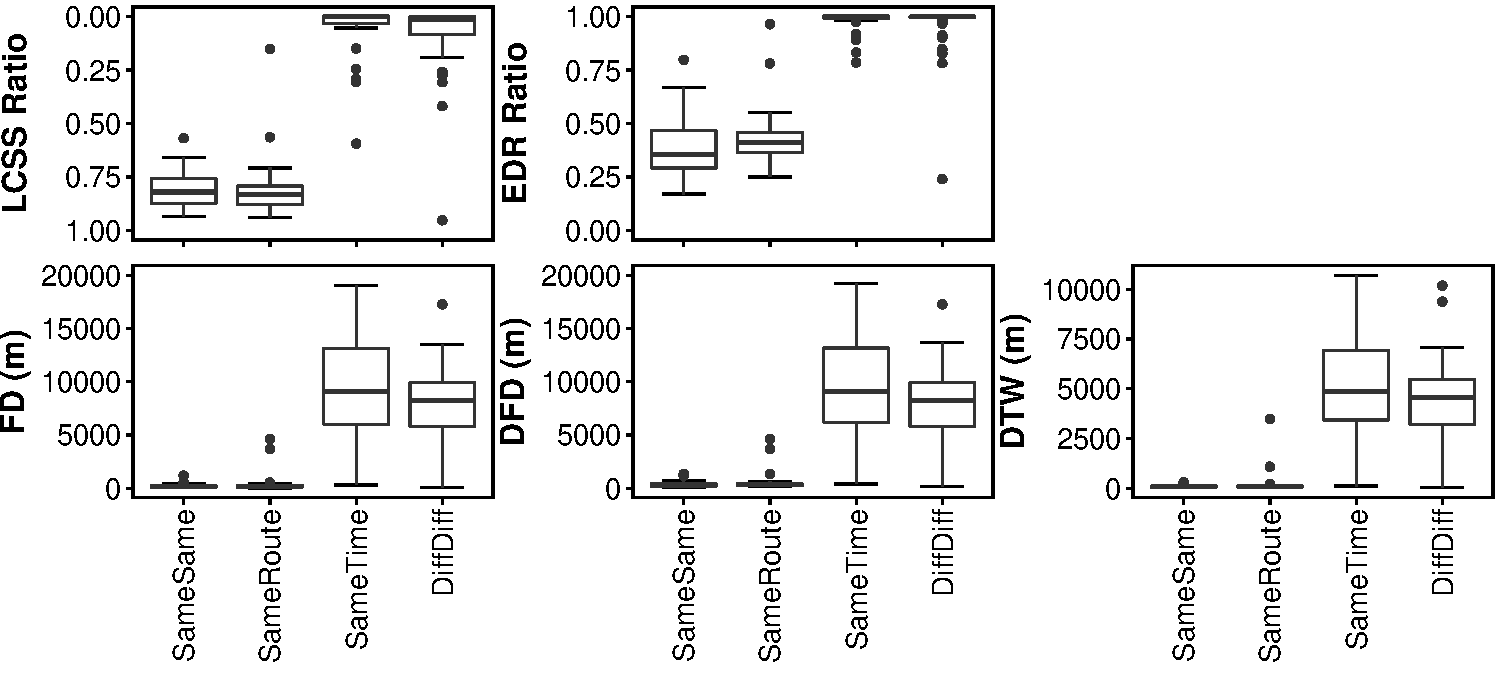
\includegraphics[width=\linewidth]{figures/Exp2}
	\caption{Box plots of bus trajectory similarity} \label{fig:bus_all}
\end{figure}

% \begin{table}[ht]
% 	\centering
% 	\caption{P-values for the Wilconxon signed rank tests on SameSame vs. SameRoute and DiffDiff vs. SameTime from Figure~\ref{fig:bus_all}).}
% 	\begin{tabular}{|c|c|c|}
% 		\hline
% 		& {\bf SameSame vs. SameRoute} & {\bf DiffDiff vs. SameTime} \\ \hline
% 		{\bf LCSS Ratio} & $0.4463$ & $0.1864$ \\ \hline
% 		{\bf EDR Ratio} & $0.0743$ & $0.7368$ \\ \hline
% 		{\bf Fréchet} & $0.6694$ & $0.1763$ \\ \hline
% 		{\bf Discrete Fréchet} & $0.2592$ & $0.1763$ \\ \hline
% 		{\bf DTW} & $0.4507 $ & $0.1115$ \\ \hline
% 	\end{tabular}
% 	\label{tab:bus_same_route}
% \end{table}

\subsection{Experiment 3: Bird behaviours}
\label{par:result_3}
In our third set of experiments, we explored the ability of similarity measures to discriminate between different activities with clear spatiotemporal signatures (cf. Fig.~\ref{fig:illu_flight_forage}). Box plots showing the results for all five similarity measures are  shown in Fig.~\ref{fig:bird_activity}. It was expected that trajectories governed by the same activity would be more alike, whereas trajectories for different activities would show greater difference.

\begin{figure}[ht]
	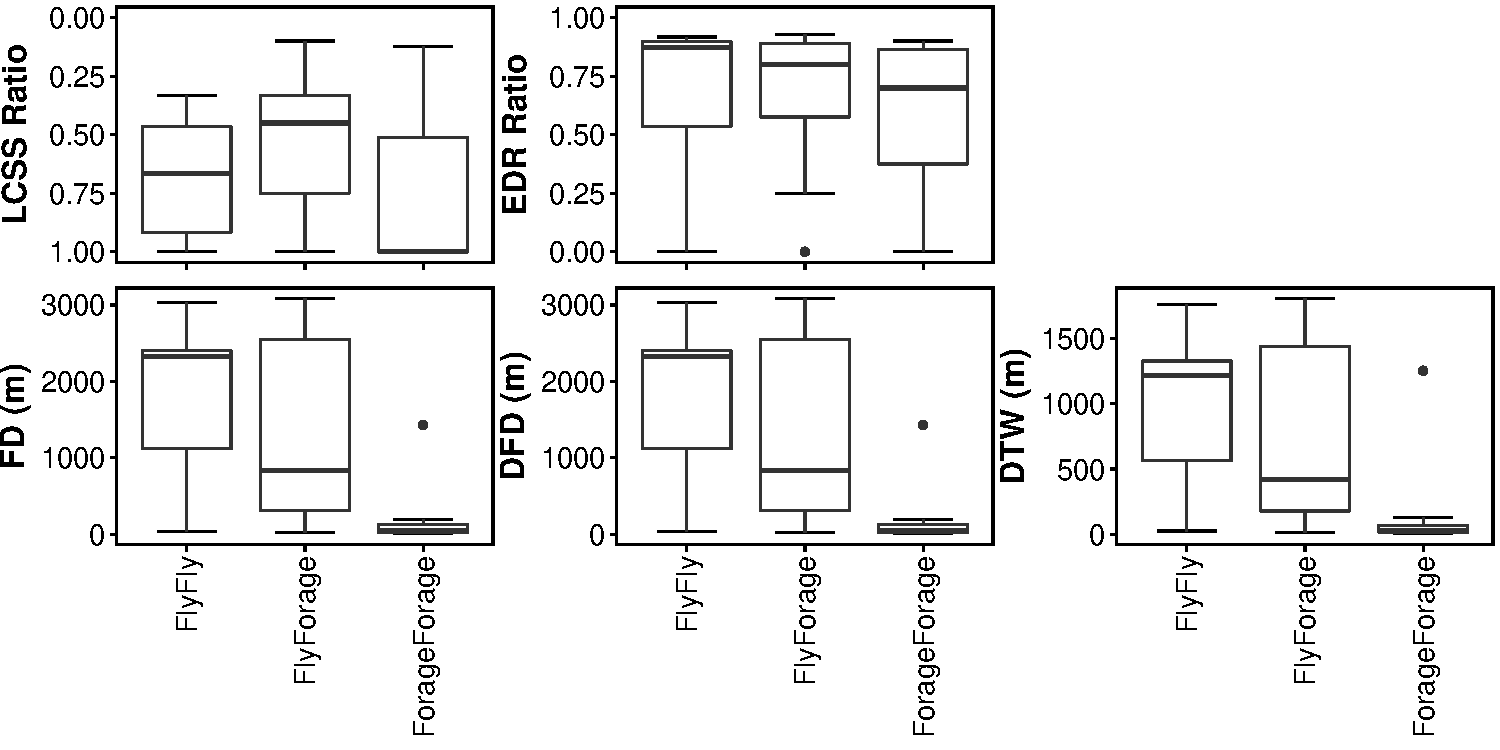
\includegraphics[width=\linewidth]{figures/Exp3}
	\caption{Box plots of bird activity trajectory similarity} \label{fig:bird_activity}
\end{figure}

In contrast to the previous experiment, the results do show a clear difference between the five similarity measures. While pairs of foraging trajectories were ranked with higher similarity by Fréchet distance, DFD, and DTW, this was not the case for pairs of flight trajectories, which were in fact at least as dissimilar than pairs of flying and foraging trajectories. The indication is that for these measures foraging trajectories do share common features that are invariant to transformation; however, one flight trajectory may as dissimilar from other flight trajectories as it is from foraging trajectories. The results for EDR indicate it is unable to distinguish any of the exhibited movement patterns, with all combinations of patterns approximately equally dissimilar. The LCSS ratio is the only measure that appear to exhibit the expected signal---that pairs of flying and pairs of foraging trajectories have greater similarity than mixed pairs---albeit a signal that is weak.

To test whether similarity measures could be treated as being drawn from different populations, according to the semantics of the comparisons, we performed a Kruskal-Wallis rank sum test (Table~\ref{tab:kruskal_wallis}). As suggested by the box plots, we found significant differences (p$<$0.05) between the similarity values for Fréchet distance, DFD, and DTW only. To further explore the nature of these differences, we then performed pairwise Wilcoxon signed rank tests to compare the (FlyFly with FlyForage/ForageForage with FlyForage) (Table~\ref{tab:wilcoxon_oyster}). We found significant differences (p$<$0.05) for both measures when comparing foraging behavior with mixed groups of trajectories, but were not able to distinguish between flying behavior from mixed groups. These results, given our previous experiment, imply that the form of trajectories has an influence on the sensitivity of measures to differences.

\begin{table}[ht]
	\centering
	\caption{P-values for Kruskal-Wallis test performed on the similarity distribution for analysis on Oystercatcher data.}
	\begin{tabular}{l|rl}
		& P-value& Significant at 5\% level\\ \hline
		LCSS Ratio & $0.3389$\  \\
		\rowcolor{gray!15} EDR Ratio & $0.5583$\ & \\
		Fréchet & $0.0057$ & * \\
		\rowcolor{gray!15} Discrete Fréchet & $0.0057$ & * \\
		DTW & $0.0075$ &* \\
	\end{tabular}
	\label{tab:kruskal_wallis}
\end{table}

\begin{table}[ht]
	\centering
	\caption{P-values for Wilcoxon signed rank tests for analysis on Oystercatcher data.}
	\begin{tabular}{l|lrl}
		& Comparison groups & P-value& Significant at 5\% level\\ \hline
		\multirow{2}{*}{FD, DFD} & {FlyVsFly and FlyVsForage} & $0.4375$ & \\
		&  {ForageVsForage and FlyVsForage} & $0.0210$ & *\\ \hline
		\multirow{2}{*}{DTW} & {FlyVsFly and FlyVsForage} & $0.5625$ & \\ 	
		& {ForageVsForage and FlyVsForage} & $0.0210$ & *\\ 	
	\end{tabular}
	\label{tab:wilcoxon_oyster}
\end{table}


\subsection{Experiment 4: Buses vs Birds}
\label{par:result_4}
Our fourth experiment compared trajectories from across our two data sets, to explore whether the similarity measures detect differences between fundamentally different types of behavior (buses moving in a structured network space versus birds free to move in a potentially unconstrained space). %This experiment provides a baseline for all experiments by comparing trajectories from very different domains that are expected to be intrinsically very different (bus movement and bird movement).

Figure~\ref{fig:BusBird} shows box plots for trajectories selected from pairs of similar (\textit{BusBus} and \textit{BirdBird}) and dissimilar (\textit{BusBird}) trajectories. Here we note that Fréchet distance, DFD, and DTW all appear to be able to discriminate between semantically similar and dissimilar objects, with largest values (and thus most dissimilar) trajectories associated with the \textit{BusBird} pairs. However, LCSS and EDR, while finding the greatest similarity between \textit{BirdBird} pairs, found either higher dissimilarity (LCSS) or  comparably high dissimilarity (EDR) between \textit{BusBus} and \textit{BusBird} pairs. As for Experiment 3, pairwise Wilcoxon signed rank tests were performed in order to determine if there was a significant difference between the three groups of trajectory pairs. With the exception of the EDR ratio on \textit{BusBird} and \textit{BusBus} trajectory pairs, all other comparisons  deferred exhibit significant differences at the 5\% level.

\begin{figure}[h]
	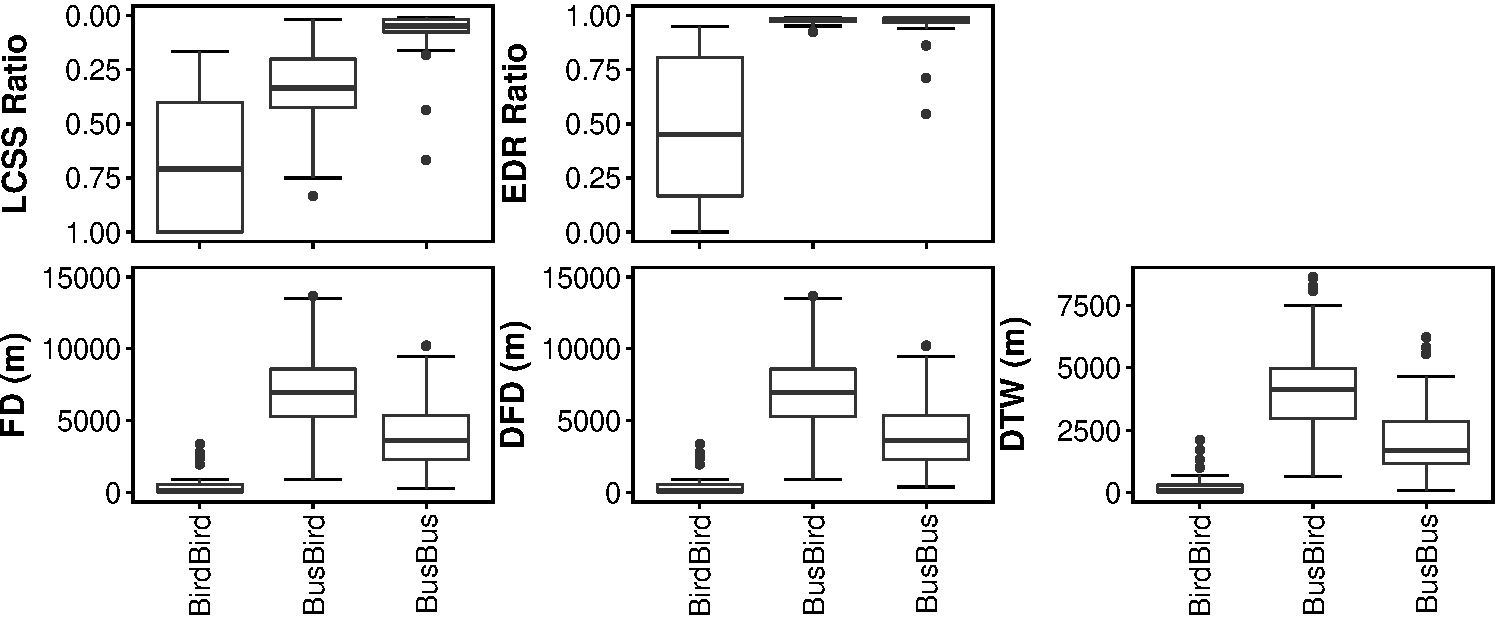
\includegraphics[width=\linewidth]{figures/Exp4}
	\caption{Box plots of bird and bus activity trajectory similarity} \label{fig:BusBird}
\end{figure}

\subsection{Lessons learned from the experimental results}

Based on the observed differences across our four experiments, we infer three general empirical properties of the different similarity measures.

\begin{enumerate}

\item Differences in similarity values are sensitive to the choice of measure. The relative ordering of similarity  for a fixed set of trajectories can be expected to differ under different similarity measures.

\item All tested similarity measures are better at distinguishing spatially dissimilar trajectories, when compared with temporally dissimilar trajectories. Relatively small spatial differences in trajectories tend to correspond to large differences in the magnitude of  measured similarity than even  relatively large temporal differences in trajectories.

\item Broadly speaking DTW, DFD, and FD tended to outperform LCSS and EDR in our experiments.  In Experiment 3, LCSS and EDR both failed to distinguish trajectories that arose from quite different activities, and were at least visually quite distinct (Fig.~\ref{fig:illu_flight_forage}). In Experiment 4, the similarity values for EDR even failed to enable discernment apart the dissimilarity between different bus trajectories when compared with the dissimilarity between bus and bird trajectories.
\end{enumerate}
 	
\section{Conclusions and recommendations}
\label{sec:discussion}

% Orphan 

%\subsection{A key to choosing a suitable similarity measure}

Table \ref{tab:key} provides a visual summary of the most salient differences between the similarity measures. The table  indicates for each similarity measure whether it is a metric; operates on continuous trajectories; temporally aligns trajectories; can be used with a distance measure that is invariant under transformation (relative space using invariant distance); the relative computational efficiency;  and the measure robustness to outliers. Note that for the last two categories more stars indicate better performance.

\begin{table}[htb]
    \caption{Summary of differences in similarity measures}\label{tab:key}
\renewcommand{\arraystretch}{2}
    \begin{tabular}{>{\raggedright\arraybackslash}p{2.8cm}|>{\raggedright\arraybackslash}p{1.25cm}>{\raggedright\arraybackslash}p{1.25cm}>{\raggedright\arraybackslash}p{1.25cm}>{\raggedright\arraybackslash}p{1.25cm}>{\raggedright\arraybackslash}p{1.25cm}p{1.25cm}}
~                                        & LSED     & DTW         & EDR         & LCSS        & DFD      & FD      \\ \hline
    Metric?                                  & Yes      & \cellcolor{gray!30}  No          & \cellcolor{gray!15} No, but see \cite{NgC04}& \cellcolor{gray!30} No          & Yes      & Yes     \\
    Continuous?                              & \cellcolor{gray!30} No       & \cellcolor{gray!15} No, but see \cite{b-cfdts-07} & \cellcolor{gray!30} No          & \cellcolor{gray!15} No, but see \cite{bbw-09} & \cellcolor{gray!30} No       & Yes     \\
    Relative time?                           & \cellcolor{gray!30}  rigid       & \cellcolor{gray!15} semi-flexible         & \cellcolor{gray!15} semi-flexible         & \cellcolor{gray!15} semi-flexible        & flexible      & flexible     \\
    Computational efficiency?                & $\star\star\star$  & \cellcolor{gray!15} $\star\,\star$    & \cellcolor{gray!15} $\star\,\star$    & \cellcolor{gray!15}$\star\,\star$    & \cellcolor{gray!15}$\star\,\star$ & \cellcolor{gray!30}$\star$ \\
    Outliers?                                & \cellcolor{gray!15}$\star\,\star$ & \cellcolor{gray!15}$\star\,\star$    & $\star\star\star$        & $\star\star\star$        & \cellcolor{gray!30} $\star$     & \cellcolor{gray!30} $\star$    \\
    \end{tabular}
\end{table}
% You may title this section "Methods" or "Models".
% "Models" is not a valid title for PLoS ONE authors. However, PLoS ONE
% authors may use "Analysis"
	

\paragraph*{Metric measures}  Some applications, such as indexing or clustering, rely on similarity measures that offer metric properties. In such cases only some of these similarity measures are suitable (LSED, DFD, FD, and possibly edit distance, although not EDR).
 	
\paragraph*{Discrete vs continuous measures} Only Fréchet distance, and its interpolation between measured locations, can provide a measure of difference over continuous trajectory paths, although some continuous analogs of DTW and LCSS can also offer continuous measure properties. The decision as to whether to use a discrete or a continuous measure usually depends on several aspects, such as whether the sampling rates in the trajectories are expected to be similar (in density, meaning of the sampling points, etc.); whether interpolation between trajectory points is possible and meaningful; and the fact that discrete measures are typically simpler to implement.

\paragraph*{Computational efficiency} A major factor to consider when selecting a similarity measure is computational efficiency. In theory, FD is the least efficient measure; LSED the most efficient; with DTW, LCSS, EDR, DFD all underpinned by similar dynamic programming implementations. However, in practice throughout all of the experiments, little to no difference was found when comparing FD to its discrete counterpart. In all cases, the primary influence in execution time is the number of sample points in the trajectories, meaning that over-sampling should be avoided.

\paragraph*{Maximum vs sum of distances} %(or: wide/narrow perspective, holistic/atomistic, instantaneous/global)
Similarity measures at root measure either the \textit{maximum} of distance between trajectories (i.e., FD, DFD), or the \textit{sum} of all or a sample of distances  between trajectories (LSED, DTW, EDR, LCSS). Different measures in this respect may lend themselves to different applications. As a direct consequence, those measures that are based on maximum distances are much more sensitive to outliers than those based on the sum of distances. That said, in our experiments FD, DFD, and DTW performed similarly, indicating that any outliers present in our data sets were not sufficiently significant to influence the results.
 	
\paragraph*{Spatial vs temporal similarity}
In all of the similarity measures tested, the spatial differences between trajectories were more important in determining the magnitude of measured similarity than temporal differences. This is particularly evident in Experiment 2. However, the precise  magnitude of these differences is likely to depend strongly on the specific application.

\paragraph*{Thresholds} This exploration has not  covered the selection of meaningful thresholds  for similarity  measures that require them, EDR and LCSS. Neither theory nor the experiments in this  paper can offer insights into the right thresholds to choose. Thresholds are highly data dependent,  and their selection needs to take into account the specific characteristics of the application, including noise, outliers, and constrained or unconstrained spaces for movement.

\paragraph*{Bounded versus unbounded measures}
As noted among the five similarity measures, LCSS and ED can be expressed as ratios, bounded between $0$ and $1$. Fréchet distance, DFD, and DTW are unbounded positive numbers. Though bounded measures do enable similarity results to be compared across different data sets, they have low resolution when representing high dissimilarity. For example, while it is easy to define 0 in edit distance ratio as two trajectories that are identical, there is no situation where two trajectories are so different that they produce a value of $1$. Additionally, the lower discriminatory power poses significant issues when different types of trajectories are compared as evidenced by LCSS and EDR ratio's inability to distinguish different movement patterns in Experiment 3.

\bigskip

In summary, as argued in Section~\ref{sub:conceptual}, our aim was not to promote a single similarity measure that fits all situations; rather  our aim is to clarify and illuminate the important differences and similarities between measures. The decision on which similarity measure to apply depends on each individual definition of distance, with different applications placing  the emphasis on different aspects of the trajectories they compare. The conceptual, theoretical, and experimental characteristics of the most popular measures, thoroughly explored in this paper, are we believe a fundamental evidence-base for making that decision. 

\section*{Data and code availability statement}

The data and codes that support the findings of this study are available with the identifiers at the following links: 
\href{https://doi.org/10.1371/journal.pone.0037997.s006}{https://doi.org/10.1371/journal.pone.0037997.s006} (Oystercatcher data),
\href{https://figshare.com/s/9fd95ce98b7ab5f4642c}{https://figshare.com/s/9fd95ce98b7ab5f4642c} (Dublin bus GPS data), and \href{https://figshare.com/s/24b7797cd30b00b45bcf}{https://figshare.com/s/24b7797cd30b00b45bcf} (code).  

% \paragraph*{General versus specific patterns}
%Despite various levels of transformation, trajectories tend to be more diverse when they are clustered based on a more general pattern. For example, bus trajectories of the same route show a high degree of similarity with each other, whereas one bird trajectory in general can be quite different from another bird trajectory. Additionally, even for the same level of abstraction, some patterns are simply  harder to extract using the discussed similarity measures. The diversity of trajectories for flight activity as opposed to foraging activity shown by experiment 3 is a clear example of this.


%	\section{Conclusion} % (fold)
%	\label{sec:Conclusion}
%	Triggered by the hardness of a decision, which one has to make in choosing a suitable similarity measure for more complicated trajectory mining tasks, six trajectory similarity measures were evaluated and compared in great detail in theoretical definitions.
%	Four among them were then evaluated on trajectories with various levels of transformation being allowed.
%	With hoping variation in transformation can represent the essences for most application scenarios, all four measures seem applicable for trajectory comparison allowing temporal transformation while Fréchet distance and DTW ratio show advantages in extracting similarity from activities when both spatial and temporal transformation are allowed.
%	Admittedly, the type of transformation is highly subject to application scenarios and so is the choice for similarity measure.

%\rodrigo{In relation to the comment about page 5: a new paragraph ``Location vs other features'', saying we did not look at that, but there are many combinations of location, direction, etc. (we could cite measures that combine these things)}

% Do NOT remove this, even if you are not including acknowledgments.

%\section*{Acknowledgments}
%This work was initiated as a result of a Lorentz Center Workshop, \textit{Geometric Algorithms in the Field}, 23--27 June 2014, at Leiden University, Netherlands. Prof. Duckham and Dr. Both receive research funding support from the Cooperative Research Centre for Spatial Information (CRCSI) under the Rapid Spatial Analytics Program.
%R. Silveira is supported by projects MINECO MTM2015-63791-R and Gen.\ Cat.\ 2017SGR1640. P. Laube thanks the Institute of Natural Resource Sciences at the Zurich University of Applied Sciences (ZHAW) for supporting his research.


\nolinenumbers

% Either type in your references using
% \begin{thebibliography}{}
% \bibitem{}
% Text
% \end{thebibliography}
%
% or

\bibliography{trajectory_similarity}


\end{document}

